%! Author = serox
%! Date = 08/12/2024


\chapter{Mesures}


\section{Méthodologie}


\section{Analyse des résultats}


\begin{table}[h!]
    \centering
    \label{tab:comparaison_materiaux}
    \renewcommand{\arraystretch}{1.5}
    \begin{tabular}{|p{4cm}|p{4cm}|p{4cm}|}
        \hline
        \textbf{Matériau} & \textbf{Force maximale avant rupture (N)} & \textbf{Allongement maximal avant rupture (\%)} \\ \hline
        Fibre de carbone  & $21\ 149 \pm 106$                         & $0,673 \pm 0,003$                               \\ \hline
        Fibre de verre    & $10\ 286 \pm 52$                          & $1,84 \pm 0,01$                                 \\ \hline
        Aluminium         & $9\ 584 \pm 48$                           & $9,54 \pm 0,05$                                 \\ \hline
    \end{tabular}
    \caption{Comparaison des propriétés mécaniques des matériaux testés}
\end{table}

\begin{figure}[!htb]
    \centering
    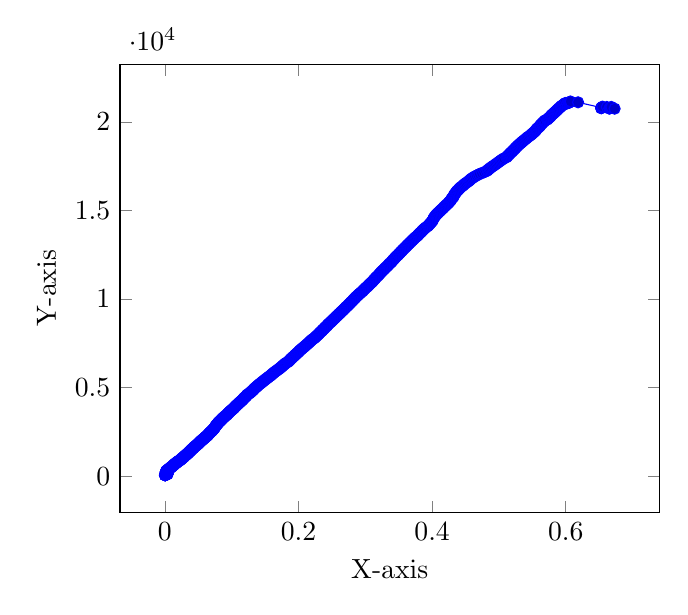
\begin{tikzpicture}
    \begin{axis}[
        xlabel={X-axis},
        ylabel={Y-axis}
    ]
        \addplot coordinates {
            (0,58.1180038452148)
            (0.000181996050429358,57.7992668151855)
            (0.000396029297240692,57.9794960021973)
            (0.0003722525045759,57.9371070861816)
            (0.000237609242728868,58.2010765075684)
            (0.000340537748120779,58.5957221984863)
            (0.000562219820681064,59.5517234802246)
            (0.000412119585783059,61.0890464782715)
            (0.000546498084598015,64.8297729492187)
            (0.000641544969859626,70.6276245117187)
            (0.000887084379853849,76.7926635742187)
            (0.00144146234558031,82.8473510742187)
            (0.0016001323526251,88.3331909179687)
            (0.00220985700861714,93.8126831054687)
            (0.00269316202659016,99.3126831054687)
            (0.0030338178819201,104.660339355469)
            (0.00331101384977411,109.662292480469)
            (0.00354096647022905,113.984558105469)
            (0.00384968242633067,119.234069824219)
            (0.00369128671784479,128.461608886719)
            (0.00403988540617025,135.832366943359)
            (0.00369162130180125,143.340179443359)
            (0.00370719301999114,150.663421630859)
            (0.00341402420418655,158.116546630859)
            (0.00310513527536731,165.639984130859)
            (0.00290711351133105,172.226898193359)
            (0.00262991197867112,178.620452880859)
            (0.00252698532821451,185.816741943359)
            (0.00187748610591387,192.654632568359)
            (0.00153674654662809,199.775726318359)
            (0.001457495362995,207.458343505859)
            (0.00140977634062249,216.269866943359)
            (0.0011325636783507,226.035491943359)
            (0.00129892378345507,236.676116943359)
            (0.00170321748411721,247.197601318359)
            (0.00163977313172449,258.334320068359)
            (0.00239196041342754,269.226898193359)
            (0.00225745534426107,280.101898193359)
            (0.00224155483878757,288.947601318359)
            (0.00224158057601499,293.590179443359)
            (0.00201996496230884,289.156890869141)
            (0.00200386574689029,293.568511962891)
            (0.00274875582901901,302.879058837891)
            (0.00297841768836418,314.238433837891)
            (0.00304179248068279,326.652496337891)
            (0.00382555157288867,340.103668212891)
            (0.00401597204389329,354.117340087891)
            (0.00470526925106081,368.330230712891)
            (0.0050456855878689,382.629058837891)
            (0.00526001965301739,396.634918212891)
            (0.00586980366693934,411.287261962891)
            (0.00632909909786621,425.480621337891)
            (0.00690747534712677,439.410308837891)
            (0.00750135143583398,453.963043212891)
            (0.00794537703929259,467.443511962891)
            (0.00839670691426641,479.636871337891)
            (0.00859499207911663,489.007965087891)
            (0.00868973846485809,496.559722900391)
            (0.00929178183373327,506.284332275391)
            (0.00970372308487633,517.137878417969)
            (0.0100681112144236,529.024963378906)
            (0.0105671630101064,540.821838378906)
            (0.010765205178431,554.323791503906)
            (0.0112721923873681,567.687072753906)
            (0.0116366797559544,581.062072753906)
            (0.0120962288492849,595.773010253906)
            (0.0123650609138281,608.944885253906)
            (0.0129990416313955,621.413635253906)
            (0.0133636440059711,634.075744628906)
            (0.0135455482371026,646.079650878906)
            (0.013870354829547,657.903869628906)
            (0.0139972713583621,669.521057128906)
            (0.0146784091688367,681.239807128906)
            (0.0149000127254633,692.222229003906)
            (0.0152406678851925,703.200744628906)
            (0.0156049716151833,713.909729003906)
            (0.0163965485641182,724.827697753906)
            (0.0165317659284435,736.138244628906)
            (0.0167776264741132,746.439025878906)
            (0.0170232495880633,756.823791503906)
            (0.0173242703450332,767.484130859375)
            (0.0179894186131394,777.866943359375)
            (0.0181006127102707,788.189208984375)
            (0.0185834894700541,797.818115234375)
            (0.0188055419210257,807.521240234375)
            (0.0190667279422229,818.488037109375)
            (0.0194232706228785,828.152099609375)
            (0.0199381413068811,838.764404296875)
            (0.0203421907357497,848.973388671875)
            (0.0209363636141064,858.125732421875)
            (0.0210477190906096,868.055419921875)
            (0.0213878400289697,879.119873046875)
            (0.021997805826552,889.899169921875)
            (0.022631475842455,901.364013671875)
            (0.0229007827704375,912.752685546875)
            (0.023360925443067,923.494873046875)
            (0.0236536787533623,934.959716796875)
            (0.0238909194146485,947.719482421875)
            (0.0244059718823114,959.412841796875)
            (0.0245322966867628,971.229248046875)
            (0.025158645272999,983.697509765625)
            (0.0255625444521075,995.488525390625)
            (0.0259110348585843,1006.66235351562)
            (0.025919014790286,1020.02368164062)
            (0.0265448124607353,1030.64282226562)
            (0.0267663826285264,1040.82641601562)
            (0.0272498585324148,1053.29516601562)
            (0.0278040668295272,1065.77172851562)
            (0.027994427710735,1078.36352539062)
            (0.0285411123902318,1091.93188476562)
            (0.0286361036274341,1103.66821289062)
            (0.0291904250756004,1115.33422851562)
            (0.0293567459951963,1127.82446289062)
            (0.0297210868238932,1140.26196289062)
            (0.0301648949361868,1153.70336914062)
            (0.0304580693167973,1166.57250976562)
            (0.0311155752514282,1179.80297851562)
            (0.0314956960148035,1194.41821289062)
            (0.0319392963743424,1208.57055664062)
            (0.0322085773332305,1222.07250976562)
            (0.0327155237335907,1236.67407226562)
            (0.0333012677859008,1251.20922851562)
            (0.0334919254567582,1266.25219726562)
            (0.034117762080849,1281.77563476562)
            (0.0346407054433188,1295.35571289062)
            (0.0349811194614578,1310.02563476562)
            (0.0351554499917204,1324.89672851562)
            (0.0357492667224977,1340.31079101562)
            (0.0362088121059575,1355.71118164062)
            (0.0365258390997136,1371.79321289062)
            (0.0369298625594879,1386.70141601562)
            (0.0372305216040724,1400.61938476562)
            (0.0377535651330489,1415.83032226562)
            (0.0382367980404118,1430.59204101562)
            (0.0387440115514566,1446.58032226562)
            (0.0389260845817013,1462.96313476562)
            (0.0393617309786328,1477.64086914062)
            (0.0397570214029697,1492.33227539062)
            (0.0400193240952232,1507.66821289062)
            (0.0407004563408919,1523.28149414062)
            (0.0409615162264881,1538.90966796875)
            (0.0414453019045732,1553.74951171875)
            (0.0422768360150113,1569.65966796875)
            (0.0425224220302551,1585.99169921875)
            (0.043226967269401,1601.46044921875)
            (0.043108499970921,1616.88232421875)
            (0.0435363704790348,1632.13623046875)
            (0.0439639108086636,1647.62451171875)
            (0.0445265349472754,1662.58544921875)
            (0.0449703096707334,1677.60888671875)
            (0.0456038776651945,1692.17919921875)
            (0.045872453748665,1706.82763671875)
            (0.0465066783902256,1721.82568359375)
            (0.0470376016843972,1735.59130859375)
            (0.0473463705061551,1750.50537109375)
            (0.0476951985108582,1764.76708984375)
            (0.0483290558752276,1779.59130859375)
            (0.0486697221645686,1794.22998046875)
            (0.0492871633514484,1809.06591796875)
            (0.0494851814056141,1822.71240234375)
            (0.0500636763707344,1836.55163574219)
            (0.050356796958221,1852.08483886719)
            (0.0507607684798065,1866.62390136719)
            (0.0512359101593491,1881.54968261719)
            (0.0515216035858562,1896.02038574219)
            (0.0519172872564787,1909.93054199219)
            (0.0520914471326928,1923.26647949219)
            (0.0527649333350155,1936.53601074219)
            (0.0529946002954328,1950.33483886719)
            (0.0534539935741972,1964.01257324219)
            (0.0538105566591412,1978.66296386719)
            (0.0540877173832243,1992.29382324219)
            (0.0543806747364036,2006.45397949219)
            (0.0550857764561423,2020.33483886719)
            (0.0553230597809407,2033.86218261719)
            (0.0559887144463864,2048.49877929687)
            (0.056567216831248,2062.18627929687)
            (0.0568523723265153,2077.54565429687)
            (0.0572247839787441,2092.44018554687)
            (0.0578425219552734,2105.89135742187)
            (0.0582939724010424,2120.46655273437)
            (0.0590146036391927,2134.16186523437)
            (0.0590069464662349,2148.19506835937)
            (0.0594347910052544,2163.24584960937)
            (0.0599575562939345,2177.44897460937)
            (0.0601950176925225,2191.88256835937)
            (0.060694169654712,2204.42358398437)
            (0.0610902651209732,2217.85913085937)
            (0.0611855939564019,2231.68139648437)
            (0.0620170649990394,2245.81225585937)
            (0.0624528152723482,2261.36889648437)
            (0.0631094920508957,2275.03100585937)
            (0.0632212778723908,2289.83959960937)
            (0.0637759480483952,2305.11303710937)
            (0.0643377708549533,2320.30444335937)
            (0.0646074339305152,2336.14819335937)
            (0.0647421615919188,2351.18725585937)
            (0.0650986801584153,2367.38256835937)
            (0.0655897408927845,2381.82983398437)
            (0.0658667643516547,2397.84545898437)
            (0.0662634830761799,2412.60717773437)
            (0.0668254691170453,2427.34741210937)
            (0.0669523170132539,2443.28881835937)
            (0.0674273882052547,2458.88256835937)
            (0.0680690474275361,2475.98413085937)
            (0.0683940172542877,2492.25366210937)
            (0.0687345165994509,2509.03100585937)
            (0.069566225073808,2524.86694335937)
            (0.0697563782022611,2540.95288085937)
            (0.0704138859918273,2557.45288085937)
            (0.070778165607659,2573.94506835937)
            (0.07092084723167,2591.33959960937)
            (0.0711979523076938,2607.04467773437)
            (0.0719742353150015,2623.04467773437)
            (0.0724184255439688,2638.43920898437)
            (0.0725360432820771,2654.85327148437)
            (0.0731152653818388,2671.38452148437)
            (0.0733607104219992,2689.01342773437)
            (0.0736856950882332,2705.43530273437)
            (0.0741450067498441,2721.97045898437)
            (0.0744459885531725,2737.86206054687)
            (0.0747390089741523,2755.26440429687)
            (0.0748895481041346,2772.89331054687)
            (0.0752856955085844,2791.54565429687)
            (0.0755787530282704,2809.47924804687)
            (0.0759823721121472,2828.27221679687)
            (0.0765054935484067,2846.30346679687)
            (0.0765451669048075,2864.11987304687)
            (0.0769020564583659,2883.04565429687)
            (0.0774007224275043,2900.60815429687)
            (0.0777569961425399,2919.77221679687)
            (0.0784861489535024,2939.36987304687)
            (0.0786761388476483,2958.15502929687)
            (0.0791988225191747,2977.01831054687)
            (0.0794602571017035,2995.73706054687)
            (0.0798322013102342,3014.28784179687)
            (0.0803949961028945,3033.27221679687)
            (0.0808227812839842,3052.87768554687)
            (0.0812030949606316,3072.01049804687)
            (0.0819474953398387,3090.97143554687)
            (0.0824387935059274,3109.4365234375)
            (0.0828822046620648,3127.9951171875)
            (0.0835319439825545,3146.8154296875)
            (0.083991337261319,3165.8505859375)
            (0.0843318662854471,3185.3583984375)
            (0.0850923749228823,3205.8427734375)
            (0.0853457887651325,3224.4599609375)
            (0.0858922749665512,3242.7763671875)
            (0.0865499163114597,3263.1201171875)
            (0.0867162223915732,3281.3583984375)
            (0.0875555435204407,3300.9716796875)
            (0.0881418811520499,3321.1474609375)
            (0.0888550073219378,3340.3583984375)
            (0.0891876417413885,3361.2646484375)
            (0.0898609980982395,3381.5380859375)
            (0.0905105519251983,3401.0888671875)
            (0.0911838192451545,3419.9716796875)
            (0.0918255971832957,3441.2646484375)
            (0.0926968528784525,3461.6435546875)
            (0.0931881584642825,3483.7685546875)
            (0.0934891551070934,3506.01147460937)
            (0.0939557677940827,3526.47631835937)
            (0.0947090496035518,3547.04663085937)
            (0.0953029850501889,3566.85913085937)
            (0.0956833729242488,3588.52709960937)
            (0.0961746562508551,3609.77319335937)
            (0.0968320156455966,3631.04663085937)
            (0.0975369875198637,3652.15209960937)
            (0.0978379915824158,3672.40600585937)
            (0.0987169267097542,3693.27709960937)
            (0.0993747312889699,3714.48803710937)
            (0.0999449977610571,3736.99584960937)
            (0.10082408128322,3759.30834960937)
            (0.101426415876939,3781.33569335937)
            (0.101941026869998,3804.05053710937)
            (0.102813172934104,3825.90600585937)
            (0.103588981077972,3849.02709960937)
            (0.10393765697798,3872.02319335937)
            (0.104222634399458,3895.03100585937)
            (0.105133719265581,3918.16772460937)
            (0.105807416930529,3942.11352539062)
            (0.106139702622142,3966.41430664062)
            (0.106971552071582,3990.23852539062)
            (0.107668814834703,4014.50805664062)
            (0.108191483666747,4037.97680664062)
            (0.109038758758222,4061.73852539062)
            (0.109799289654881,4086.93774414062)
            (0.11048072610994,4110.94580078125)
            (0.111011386003298,4135.27392578125)
            (0.11164508384323,4159.69189453125)
            (0.112651252693322,4182.48876953125)
            (0.113110720169499,4206.10986328125)
            (0.113863185807432,4229.97314453125)
            (0.114576163582495,4254.59423828125)
            (0.115336649960706,4278.49267578125)
            (0.116073244772131,4302.70361328125)
            (0.116516537212408,4326.45361328125)
            (0.117197973667468,4350.50048828125)
            (0.1177051129811,4375.48876953125)
            (0.118544819936512,4400.95361328125)
            (0.11887743951648,4427.27783203125)
            (0.119748628433966,4452.34814453125)
            (0.120438011431891,4478.20361328125)
            (0.121356968643469,4504.65283203125)
            (0.121887346586659,4529.85986328125)
            (0.122481793995442,4556.16845703125)
            (0.122798565008125,4582.28564453125)
            (0.123614506532351,4608.65673828125)
            (0.12474733778512,4634.77001953125)
            (0.126053509032697,4661.32861328125)
            (0.126775108547079,4686.92626953125)
            (0.127480162038499,4712.79345703125)
            (0.128454552136867,4739.19970703125)
            (0.129151429073444,4765.40283203125)
            (0.129872568563869,4792.38720703125)
            (0.130799175528663,4819.76220703125)
            (0.131717976925674,4845.93798828125)
            (0.132217058400322,4872.91064453125)
            (0.13296967243308,4900.61376953125)
            (0.133571725076631,4928.14111328125)
            (0.134403715501155,4955.89013671875)
            (0.135148182658034,4984.11669921875)
            (0.135972011367196,5011.41748046875)
            (0.13685116166703,5038.13232421875)
            (0.137643590031272,5066.45263671875)
            (0.138530634935784,5093.18310546875)
            (0.139179951331023,5120.78857421875)
            (0.140154326589909,5149.42138671875)
            (0.140986124101161,5176.84716796875)
            (0.141881597831719,5204.68310546875)
            (0.142934904297897,5231.95263671875)
            (0.143837961004001,5258.95263671875)
            (0.144637987183271,5286.56982421875)
            (0.145596276443152,5313.67529296875)
            (0.146325800241176,5340.78857421875)
            (0.147402790521387,5368.04638671875)
            (0.148297744870058,5396.31982421875)
            (0.149272105289462,5424.24560546875)
            (0.150151493021015,5451.59326171875)
            (0.150927761188841,5479.28076171875)
            (0.152099872551725,5507.3984375)
            (0.153034923182048,5537.859375)
            (0.154357803686893,5566.4765625)
            (0.155062619746594,5596.1328125)
            (0.15594214103349,5625.15625)
            (0.157281063018892,5652.796875)
            (0.158246890735871,5681.9296875)
            (0.159110697010825,5711.4921875)
            (0.159982012063912,5740.75)
            (0.160750400466542,5769.76171875)
            (0.161788095797155,5799.10546875)
            (0.16254069499043,5827.88671875)
            (0.163625698591177,5856.66015625)
            (0.164520994247946,5886.96484375)
            (0.165669599870588,5916.27734375)
            (0.166865825392496,5946.57421875)
            (0.167760942975475,5976.78515625)
            (0.169084031233075,6007.26953125)
            (0.170184838882659,6037.32421875)
            (0.171040023418294,6067.04296875)
            (0.172188732917313,6098.06494140625)
            (0.173131514918007,6127.92431640625)
            (0.174153628792019,6159.22119140625)
            (0.175183236604682,6190.79931640625)
            (0.17588845333041,6221.26025390625)
            (0.17690264292078,6251.97900390625)
            (0.177821043651764,6282.20556640625)
            (0.178914238646839,6313.68212890625)
            (0.179627275779832,6345.63525390625)
            (0.180894671459697,6377.43994140625)
            (0.182090882142123,6409.54150390625)
            (0.183682327600827,6440.05712890625)
            (0.184974267784708,6470.64306640625)
            (0.185568158712898,6501.74462890625)
            (0.186479035826267,6532.77587890625)
            (0.187358482915751,6565.18994140625)
            (0.187952833867897,6597.89306640625)
            (0.188871249438364,6629.81494140625)
            (0.189687495171981,6660.94775390625)
            (0.190915432667942,6693.90869140625)
            (0.191525305718758,6725.6025390625)
            (0.192562926851959,6758.0791015625)
            (0.193679924376925,6792.3994140625)
            (0.194575576181274,6824.3369140625)
            (0.195106295432561,6857.1728515625)
            (0.196523792477676,6890.3994140625)
            (0.197300164521878,6922.9384765625)
            (0.198100309417008,6955.5791015625)
            (0.199256661249502,6988.2744140625)
            (0.200286372938542,7021.6181640625)
            (0.200911886803889,7054.8134765625)
            (0.201791601004058,7087.8681640625)
            (0.202654843378677,7120.2197265625)
            (0.203874945627891,7151.9619140625)
            (0.20472242847212,7185.2431640625)
            (0.205792266121777,7218.3916015625)
            (0.206869256401987,7253.1572265625)
            (0.208033606715536,7287.2822265625)
            (0.209055646392136,7322.1728515625)
            (0.210085387760141,7355.3056640625)
            (0.211027917489633,7388.2099609375)
            (0.212208249925809,7423.4130859375)
            (0.213150913210642,7458.5771484375)
            (0.21414100348147,7493.0693359375)
            (0.215313367115557,7527.6474609375)
            (0.216176935958791,7562.5927734375)
            (0.217167619808918,7596.5302734375)
            (0.218046562355998,7629.0068359375)
            (0.219092152291288,7664.1083984375)
            (0.220050486069616,7698.6083984375)
            (0.221255036541194,7732.9599609375)
            (0.222545656011135,7768.0068359375)
            (0.224129459136363,7801.7490234375)
            (0.224835106207083,7835.4052734375)
            (0.225785545380734,7870.0224609375)
            (0.226657127544506,7904.7958984375)
            (0.227773887637753,7938.7177734375)
            (0.228827565090993,7975.0615234375)
            (0.229698049133061,8009.2880859375)
            (0.230720904981197,8043.6708984375)
            (0.231568387825426,8079.23681640625)
            (0.232265502193722,8114.33837890625)
            (0.233382366163347,8149.79931640625)
            (0.234515316131976,8186.67431640625)
            (0.235584500844403,8222.884765625)
            (0.236043931221874,8259.126953125)
            (0.237366945282061,8294.939453125)
            (0.238420103353414,8330.400390625)
            (0.239149285843342,8366.470703125)
            (0.239925390776859,8402.845703125)
            (0.241089755929891,8439.509765625)
            (0.242317871499641,8475.517578125)
            (0.243062516730309,8510.916015625)
            (0.243814448146873,8545.416015625)
            (0.244686356779259,8581.181640625)
            (0.245628782632373,8616.892578125)
            (0.246674090617496,8652.759765625)
            (0.248045021366599,8690.470703125)
            (0.248836856151542,8726.025390625)
            (0.249890771036502,8761.931640625)
            (0.25088086130733,8798.6240234375)
            (0.251807676024879,8834.2646484375)
            (0.252884844378878,8870.9990234375)
            (0.253891080006641,8908.6708984375)
            (0.254984749865155,8946.1083984375)
            (0.255855768128592,8983.8115234375)
            (0.257004284714339,9021.5693359375)
            (0.257915250864603,9056.9677734375)
            (0.258794608917192,9091.7099609375)
            (0.260125116916029,9129.4052734375)
            (0.260742469066014,9166.4833984375)
            (0.262097610605763,9204.2490234375)
            (0.263040362927491,9241.6943359375)
            (0.264015198210334,9277.5849609375)
            (0.26498118916162,9313.1005859375)
            (0.266018736097408,9349.2412109375)
            (0.267080204278948,9386.5771484375)
            (0.268046699772639,9423.9990234375)
            (0.26899731702008,9462.0693359375)
            (0.270027177103945,9499.0927734375)
            (0.270819338357502,9536.53125)
            (0.271999492719888,9574.390625)
            (0.273322432582663,9612.078125)
            (0.274257112225924,9651.15625)
            (0.275207729473365,9689.5)
            (0.276174254646021,9728.046875)
            (0.277394000747655,9767.84375)
            (0.278075103314358,9805.265625)
            (0.27911315479255,9843.6328125)
            (0.280340884535756,9880.8828125)
            (0.281212229267808,9918.6015625)
            (0.28208321785228,9956.71875)
            (0.28309758551644,9996.2734375)
            (0.284285515767644,10033.84375)
            (0.285022385109494,10070.4765625)
            (0.285949318542903,10108.4296875)
            (0.286884087223059,10145.5546875)
            (0.288151438384477,10183.796875)
            (0.289315862895438,10224.1640625)
            (0.290226947761562,10262.9453125)
            (0.291375523705239,10302.78125)
            (0.292904405905821,10341.5966796875)
            (0.293696418764554,10380.6826171875)
            (0.295272935703886,10420.0498046875)
            (0.296358147057388,10460.2607421875)
            (0.297110746250664,10500.5029296875)
            (0.29827514108266,10539.5498046875)
            (0.299360352436162,10579.4873046875)
            (0.300334712855566,10619.1669921875)
            (0.301387870926919,10657.5732421875)
            (0.302948865767581,10697.6748046875)
            (0.303915331582306,10737.8935546875)
            (0.304992499936306,10779.2138671875)
            (0.30593504450528,10819.6513671875)
            (0.307131314545636,10860.4013671875)
            (0.308184947480428,10900.9013671875)
            (0.309444404037169,10939.2919921875)
            (0.310482218083641,10981.0966796875)
            (0.311543626907251,11021.8544921875)
            (0.31243850705851,11063.7294921875)
            (0.313294270333962,11105.1279296875)
            (0.314624956406589,11146.626953125)
            (0.31533000989801,11187.876953125)
            (0.316304370317413,11228.322265625)
            (0.317556021306371,11271.103515625)
            (0.318863023564966,11314.119140625)
            (0.319900481463859,11356.017578125)
            (0.320843500896272,11399.033203125)
            (0.321754645120326,11439.150390625)
            (0.322792132698184,11480.525390625)
            (0.323703039490518,11521.697265625)
            (0.324827753546372,11562.337890625)
            (0.325833751742415,11604.291015625)
            (0.327156661926225,11646.275390625)
            (0.328289626734336,11687.228515625)
            (0.329192579564063,11727.666015625)
            (0.33034097743395,11769.431640625)
            (0.331545320152773,11810.900390625)
            (0.332717668947377,11852.931640625)
            (0.333882123137303,11896.947265625)
            (0.334911923863238,11939.376953125)
            (0.335791133521003,11982.55078125)
            (0.337106089742205,12024.69921875)
            (0.338563683068971,12066.56640625)
            (0.339347741965096,12108.70703125)
            (0.340377720764821,12151.25390625)
            (0.341264884385193,12194.81640625)
            (0.342469078709191,12238.83203125)
            (0.343562006593581,12282.31640625)
            (0.344465078139167,12325.48828125)
            (0.345503040580465,12368.23828125)
            (0.346643899993253,12410.33203125)
            (0.347752824839753,12452.29296875)
            (0.34922588090726,12496.24609375)
            (0.34993087504075,12538.26171875)
            (0.351206180164776,12580.83203125)
            (0.352394733674244,12622.79296875)
            (0.353115546696055,12664.07421875)
            (0.354549100061209,12706.58984375)
            (0.355459858458718,12750.41796875)
            (0.356497998973805,12793.92578125)
            (0.357710176939375,12836.5224609375)
            (0.358961442101789,12880.3349609375)
            (0.359904283460412,12922.3271484375)
            (0.361298037333565,12963.6552734375)
            (0.362288483751972,13008.2412109375)
            (0.363223341469023,13050.2490234375)
            (0.364514346765509,13094.7412109375)
            (0.365766146149291,13138.6005859375)
            (0.366772055308439,13181.7880859375)
            (0.368126603268889,13224.9755859375)
            (0.369219976337753,13268.6865234375)
            (0.370383985343205,13311.2177734375)
            (0.371556601248494,13354.3583984375)
            (0.372815939089375,13397.9990234375)
            (0.37376676408957,13440.5771484375)
            (0.375176692998622,13483.4677734375)
            (0.376507705539864,13527.6318359375)
            (0.37824244104136,13571.5693359375)
            (0.378963224384206,13615.8427734375)
            (0.380151510782989,13661.2568359375)
            (0.381371405279448,13707.27734375)
            (0.38251977347037,13752.61328125)
            (0.384072576916704,13795.81640625)
            (0.384745992631485,13839.07421875)
            (0.386156129293292,13883.61328125)
            (0.387114374034726,13928.51171875)
            (0.388571789287702,13973.28515625)
            (0.389918947185878,14019.29296875)
            (0.391352411514138,14063.28515625)
            (0.393245395256762,14106.69921875)
            (0.394465289753221,14151.12109375)
            (0.395424128073954,14194.54296875)
            (0.396485240107914,14239.00390625)
            (0.397531453301468,14284.05859375)
            (0.398648213394715,14328.87109375)
            (0.399574909396404,14373.84765625)
            (0.400683923279799,14418.19921875)
            (0.401254174912403,14460.78515625)
            (0.401349800537481,14505.44921875)
            (0.402078300411215,14549.89453125)
            (0.402822856604988,14596.1494140625)
            (0.40367826373286,14641.6884765625)
            (0.404810991109252,14687.2197265625)
            (0.40549218271285,14730.8759765625)
            (0.406688274679416,14776.6650390625)
            (0.407781380637596,14821.6337890625)
            (0.409096099427079,14867.3369140625)
            (0.410308574182299,14914.2275390625)
            (0.411694819277318,14959.7666015625)
            (0.412740142101924,15004.6650390625)
            (0.414182064935195,15050.0087890625)
            (0.415338357409759,15094.1259765625)
            (0.416819931340207,15139.5166015625)
            (0.417604257347017,15184.7822265625)
            (0.419014186256069,15229.9150390625)
            (0.420257972319314,15274.6728515625)
            (0.421414027362159,15319.7275390625)
            (0.42279303078973,15364.5791015625)
            (0.424187022094602,15408.5556640625)
            (0.425074185714973,15454.8291015625)
            (0.426111613934901,15500.4375)
            (0.427458475043428,15547.6953125)
            (0.428409211006729,15592.8515625)
            (0.42885276313795,15637.8984375)
            (0.429454800942019,15682.3828125)
            (0.430935870330063,15729.359375)
            (0.43225109366195,15774.3984375)
            (0.432013424510607,15820.15625)
            (0.432765845630093,15867.9140625)
            (0.433589258833745,15913.359375)
            (0.434492834921736,15959.078125)
            (0.435522635647671,16004.390625)
            (0.436235583743769,16049.9140625)
            (0.437130493573994,16096.03125)
            (0.438603816752185,16143.421875)
            (0.439760584090188,16189.8203125)
            (0.44086173304787,16236.359375)
            (0.442002414386869,16282.234375)
            (0.443443981072561,16327.765625)
            (0.445202400388089,16374.328125)
            (0.446667977356428,16421.08203125)
            (0.447880155321998,16469.00390625)
            (0.44950448507387,16515.99609375)
            (0.45108836239651,16562.30078125)
            (0.452957781040962,16608.29296875)
            (0.454699758209907,16655.12109375)
            (0.456063031786053,16699.23828125)
            (0.457346231514756,16745.30859375)
            (0.458811719446199,16793.44921875)
            (0.460649411277117,16839.25390625)
            (0.462589940721596,16885.12109375)
            (0.464229881609033,16930.01171875)
            (0.466661657281412,16973.20703125)
            (0.4690378739314,17019.55078125)
            (0.471367197816762,17066.02734375)
            (0.474606834915159,17113.63671875)
            (0.477815012310706,17160.82421875)
            (0.480777744666092,17209.00390625)
            (0.482892548992775,17254.32421875)
            (0.483724687812124,17299.11328125)
            (0.48549123916405,17346.53515625)
            (0.486917165035211,17393.01953125)
            (0.48861230879746,17441.55078125)
            (0.490497605688162,17488.99609375)
            (0.492343103086862,17535.52734375)
            (0.494140995425778,17580.80078125)
            (0.495646431244048,17625.16796875)
            (0.497404969275436,17671.92578125)
            (0.499139942208652,17718.68359375)
            (0.500708416148482,17765.80859375)
            (0.502593980149869,17812.08984375)
            (0.504138176696367,17857.03515625)
            (0.506007595340819,17902.83203125)
            (0.507765717866698,17948.09765625)
            (0.510983036383451,17994.37890625)
            (0.512337168838391,18040.75390625)
            (0.513406205155994,18088.52734375)
            (0.514650109935099,18136.86328125)
            (0.515885645246088,18182.93359375)
            (0.516970886278555,18229.40234375)
            (0.5182464288343,18276.40625)
            (0.519767357072275,18322.3828125)
            (0.520852776178532,18369.703125)
            (0.522159719079197,18418.0859375)
            (0.523395551179835,18465.1875)
            (0.524575764900152,18511.0390625)
            (0.525486849766275,18558.28125)
            (0.52698314446334,18603.9375)
            (0.52814828126946,18651.203125)
            (0.529582072066334,18700.3828125)
            (0.530810365709874,18746.546875)
            (0.532418134599302,18793.0234375)
            (0.533764313091635,18839.0703125)
            (0.534897396615606,18881.6875)
            (0.536497448974146,18927.640625)
            (0.537852175008385,18972.15625)
            (0.53943655687343,19018.03125)
            (0.540981109567508,19064.4140625)
            (0.542375486698924,19112.25)
            (0.543848572445396,19158.8203125)
            (0.545702023806703,19204.056640625)
            (0.547460858627741,19251.470703125)
            (0.548973714187249,19297.830078125)
            (0.550051357404689,19345.314453125)
            (0.551738131698821,19392.455078125)
            (0.55306139803021,19438.791015625)
            (0.554305065377596,19483.744140625)
            (0.555485457171702,19528.556640625)
            (0.556103017074442,19573.751953125)
            (0.556982879669435,19619.251953125)
            (0.558559010782223,19665.783203125)
            (0.55992145334735,19711.017578125)
            (0.561038213440597,19754.931640625)
            (0.562068073524462,19797.044921875)
            (0.562376912833762,19832.857421875)
            (0.563913452207302,19877.708984375)
            (0.564808569790281,19921.748046875)
            (0.565957501881537,19967.927734375)
            (0.567652408212067,20013.544921875)
            (0.568056813788515,20049.365234375)
            (0.569205449090121,20092.015625)
            (0.571906887838062,20117.603515625)
            (0.573094818089267,20161.150390625)
            (0.574275091167513,20205.009765625)
            (0.575526653119576,20250.416015625)
            (0.577063429924836,20293.830078125)
            (0.577800299266687,20337.689453125)
            (0.578829981276762,20383.298828125)
            (0.580010313712938,20426.298828125)
            (0.581602115319221,20470.337890625)
            (0.582663969327305,20515.064453125)
            (0.584042438533507,20558.626953125)
            (0.58532557890428,20603.525390625)
            (0.5866483110143,20647.720703125)
            (0.587741506009375,20690.884765625)
            (0.588906286667915,20734.884765625)
            (0.590102230239657,20779.853515625)
            (0.591757841620589,20827.697265625)
            (0.592756123285744,20870.806640625)
            (0.593880125046439,20907.888671875)
            (0.595433403356213,20938.615234375)
            (0.596787832600803,20981.802734375)
            (0.598229696076144,21026.591796875)
            (0.599330845033826,21066.232421875)
            (0.601636307031366,21043.537109375)
            (0.602403092769889,21053.556640625)
            (0.60424182336458,21072.611328125)
            (0.604646169583098,21079.6484375)
            (0.60553333320347,21110.828125)
            (0.606412661577094,21139.4375)
            (0.607490186078673,21149.10546875)
            (0.618519245602744,21106.5234375)
            (0.653830565808526,20801.3203125)
            (0.653276103385277,20781.509765625)
            (0.653086514157158,20775.4921875)
            (0.653157209451675,20783.669921875)
            (0.65397296548237,20804.677734375)
            (0.654693808183146,20829.548828125)
            (0.655121838215696,20862.146484375)
            (0.661608947659238,20843.068359375)
            (0.665316622034942,20750.482421875)
            (0.665665053083489,20765.01953125)
            (0.666481165261763,20784.28515625)
            (0.667273356194286,20814.37109375)
            (0.668413859459495,20845.3671875)
            (0.673238828149815,20747.85546875)


        };
    \end{axis}
\end{tikzpicture}

\end{figure}
\begin{figure}[!htb]
    \centering
    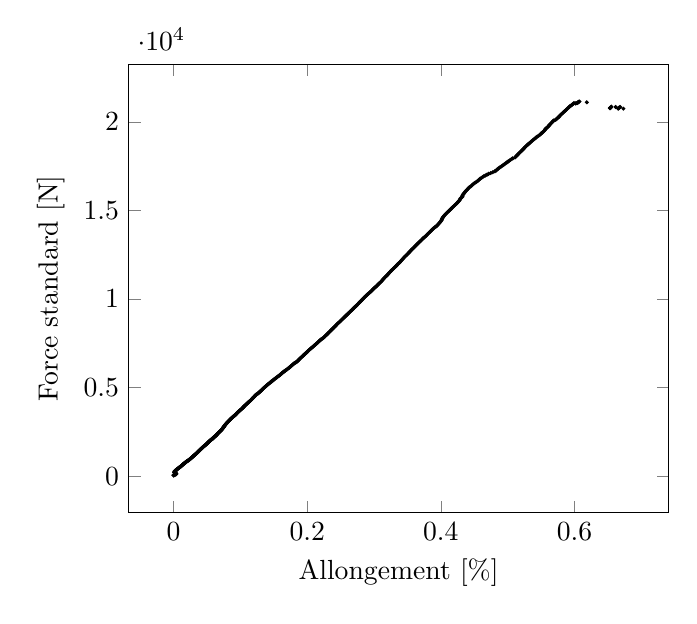
\begin{tikzpicture}
    \begin{axis}[
        xlabel={Allongement [\%]},
        ylabel={Force standard [N]}
    ]
        \addplot
[
    only marks,
    mark=*,
    mark size=0.5pt % Adjust the size here
]
 coordinates {
(0.000181996050429358,57.7992668151855)
(0.000396029297240692,57.9794960021973)
(0.0003722525045759,57.9371070861816)
(0.000237609242728868,58.2010765075684)
(0.000340537748120779,58.5957221984863)
(0.000562219820681064,59.5517234802246)
(0.000412119585783059,61.0890464782715)
(0.000546498084598015,64.8297729492187)
(0.000641544969859626,70.6276245117187)
(0.000887084379853849,76.7926635742187)
(0.00144146234558031,82.8473510742187)
(0.0016001323526251,88.3331909179687)
(0.00220985700861714,93.8126831054687)
(0.00269316202659016,99.3126831054687)
(0.0030338178819201,104.660339355469)
(0.00331101384977411,109.662292480469)
(0.00354096647022905,113.984558105469)
(0.00384968242633067,119.234069824219)
(0.00369128671784479,128.461608886719)
(0.00403988540617025,135.832366943359)
(0.00369162130180125,143.340179443359)
(0.00370719301999114,150.663421630859)
(0.00341402420418655,158.116546630859)
(0.00310513527536731,165.639984130859)
(0.00290711351133105,172.226898193359)
(0.00262991197867112,178.620452880859)
(0.00252698532821451,185.816741943359)
(0.00187748610591387,192.654632568359)
(0.00153674654662809,199.775726318359)
(0.001457495362995,207.458343505859)
(0.00140977634062249,216.269866943359)
(0.0011325636783507,226.035491943359)
(0.00129892378345507,236.676116943359)
(0.00170321748411721,247.197601318359)
(0.00163977313172449,258.334320068359)
(0.00239196041342754,269.226898193359)
(0.00225745534426107,280.101898193359)
(0.00224155483878757,288.947601318359)
(0.00224158057601499,293.590179443359)
(0.00201996496230884,289.156890869141)
(0.00200386574689029,293.568511962891)
(0.00274875582901901,302.879058837891)
(0.00297841768836418,314.238433837891)
(0.00304179248068279,326.652496337891)
(0.00382555157288867,340.103668212891)
(0.00401597204389329,354.117340087891)
(0.00470526925106081,368.330230712891)
(0.0050456855878689,382.629058837891)
(0.00526001965301739,396.634918212891)
(0.00586980366693934,411.287261962891)
(0.00632909909786621,425.480621337891)
(0.00690747534712677,439.410308837891)
(0.00750135143583398,453.963043212891)
(0.00794537703929259,467.443511962891)
(0.00839670691426641,479.636871337891)
(0.00859499207911663,489.007965087891)
(0.00868973846485809,496.559722900391)
(0.00929178183373327,506.284332275391)
(0.00970372308487633,517.137878417969)
(0.0100681112144236,529.024963378906)
(0.0105671630101064,540.821838378906)
(0.010765205178431,554.323791503906)
(0.0112721923873681,567.687072753906)
(0.0116366797559544,581.062072753906)
(0.0120962288492849,595.773010253906)
(0.0123650609138281,608.944885253906)
(0.0129990416313955,621.413635253906)
(0.0133636440059711,634.075744628906)
(0.0135455482371026,646.079650878906)
(0.013870354829547,657.903869628906)
(0.0139972713583621,669.521057128906)
(0.0146784091688367,681.239807128906)
(0.0149000127254633,692.222229003906)
(0.0152406678851925,703.200744628906)
(0.0156049716151833,713.909729003906)
(0.0163965485641182,724.827697753906)
(0.0165317659284435,736.138244628906)
(0.0167776264741132,746.439025878906)
(0.0170232495880633,756.823791503906)
(0.0173242703450332,767.484130859375)
(0.0179894186131394,777.866943359375)
(0.0181006127102707,788.189208984375)
(0.0185834894700541,797.818115234375)
(0.0188055419210257,807.521240234375)
(0.0190667279422229,818.488037109375)
(0.0194232706228785,828.152099609375)
(0.0199381413068811,838.764404296875)
(0.0203421907357497,848.973388671875)
(0.0209363636141064,858.125732421875)
(0.0210477190906096,868.055419921875)
(0.0213878400289697,879.119873046875)
(0.021997805826552,889.899169921875)
(0.022631475842455,901.364013671875)
(0.0229007827704375,912.752685546875)
(0.023360925443067,923.494873046875)
(0.0236536787533623,934.959716796875)
(0.0238909194146485,947.719482421875)
(0.0244059718823114,959.412841796875)
(0.0245322966867628,971.229248046875)
(0.025158645272999,983.697509765625)
(0.0255625444521075,995.488525390625)
(0.0259110348585843,1006.66235351562)
(0.025919014790286,1020.02368164062)
(0.0265448124607353,1030.64282226562)
(0.0267663826285264,1040.82641601562)
(0.0272498585324148,1053.29516601562)
(0.0278040668295272,1065.77172851562)
(0.027994427710735,1078.36352539062)
(0.0285411123902318,1091.93188476562)
(0.0286361036274341,1103.66821289062)
(0.0291904250756004,1115.33422851562)
(0.0293567459951963,1127.82446289062)
(0.0297210868238932,1140.26196289062)
(0.0301648949361868,1153.70336914062)
(0.0304580693167973,1166.57250976562)
(0.0311155752514282,1179.80297851562)
(0.0314956960148035,1194.41821289062)
(0.0319392963743424,1208.57055664062)
(0.0322085773332305,1222.07250976562)
(0.0327155237335907,1236.67407226562)
(0.0333012677859008,1251.20922851562)
(0.0334919254567582,1266.25219726562)
(0.034117762080849,1281.77563476562)
(0.0346407054433188,1295.35571289062)
(0.0349811194614578,1310.02563476562)
(0.0351554499917204,1324.89672851562)
(0.0357492667224977,1340.31079101562)
(0.0362088121059575,1355.71118164062)
(0.0365258390997136,1371.79321289062)
(0.0369298625594879,1386.70141601562)
(0.0372305216040724,1400.61938476562)
(0.0377535651330489,1415.83032226562)
(0.0382367980404118,1430.59204101562)
(0.0387440115514566,1446.58032226562)
(0.0389260845817013,1462.96313476562)
(0.0393617309786328,1477.64086914062)
(0.0397570214029697,1492.33227539062)
(0.0400193240952232,1507.66821289062)
(0.0407004563408919,1523.28149414062)
(0.0409615162264881,1538.90966796875)
(0.0414453019045732,1553.74951171875)
(0.0422768360150113,1569.65966796875)
(0.0425224220302551,1585.99169921875)
(0.043226967269401,1601.46044921875)
(0.043108499970921,1616.88232421875)
(0.0435363704790348,1632.13623046875)
(0.0439639108086636,1647.62451171875)
(0.0445265349472754,1662.58544921875)
(0.0449703096707334,1677.60888671875)
(0.0456038776651945,1692.17919921875)
(0.045872453748665,1706.82763671875)
(0.0465066783902256,1721.82568359375)
(0.0470376016843972,1735.59130859375)
(0.0473463705061551,1750.50537109375)
(0.0476951985108582,1764.76708984375)
(0.0483290558752276,1779.59130859375)
(0.0486697221645686,1794.22998046875)
(0.0492871633514484,1809.06591796875)
(0.0494851814056141,1822.71240234375)
(0.0500636763707344,1836.55163574219)
(0.050356796958221,1852.08483886719)
(0.0507607684798065,1866.62390136719)
(0.0512359101593491,1881.54968261719)
(0.0515216035858562,1896.02038574219)
(0.0519172872564787,1909.93054199219)
(0.0520914471326928,1923.26647949219)
(0.0527649333350155,1936.53601074219)
(0.0529946002954328,1950.33483886719)
(0.0534539935741972,1964.01257324219)
(0.0538105566591412,1978.66296386719)
(0.0540877173832243,1992.29382324219)
(0.0543806747364036,2006.45397949219)
(0.0550857764561423,2020.33483886719)
(0.0553230597809407,2033.86218261719)
(0.0559887144463864,2048.49877929687)
(0.056567216831248,2062.18627929687)
(0.0568523723265153,2077.54565429687)
(0.0572247839787441,2092.44018554687)
(0.0578425219552734,2105.89135742187)
(0.0582939724010424,2120.46655273437)
(0.0590146036391927,2134.16186523437)
(0.0590069464662349,2148.19506835937)
(0.0594347910052544,2163.24584960937)
(0.0599575562939345,2177.44897460937)
(0.0601950176925225,2191.88256835937)
(0.060694169654712,2204.42358398437)
(0.0610902651209732,2217.85913085937)
(0.0611855939564019,2231.68139648437)
(0.0620170649990394,2245.81225585937)
(0.0624528152723482,2261.36889648437)
(0.0631094920508957,2275.03100585937)
(0.0632212778723908,2289.83959960937)
(0.0637759480483952,2305.11303710937)
(0.0643377708549533,2320.30444335937)
(0.0646074339305152,2336.14819335937)
(0.0647421615919188,2351.18725585937)
(0.0650986801584153,2367.38256835937)
(0.0655897408927845,2381.82983398437)
(0.0658667643516547,2397.84545898437)
(0.0662634830761799,2412.60717773437)
(0.0668254691170453,2427.34741210937)
(0.0669523170132539,2443.28881835937)
(0.0674273882052547,2458.88256835937)
(0.0680690474275361,2475.98413085937)
(0.0683940172542877,2492.25366210937)
(0.0687345165994509,2509.03100585937)
(0.069566225073808,2524.86694335937)
(0.0697563782022611,2540.95288085937)
(0.0704138859918273,2557.45288085937)
(0.070778165607659,2573.94506835937)
(0.07092084723167,2591.33959960937)
(0.0711979523076938,2607.04467773437)
(0.0719742353150015,2623.04467773437)
(0.0724184255439688,2638.43920898437)
(0.0725360432820771,2654.85327148437)
(0.0731152653818388,2671.38452148437)
(0.0733607104219992,2689.01342773437)
(0.0736856950882332,2705.43530273437)
(0.0741450067498441,2721.97045898437)
(0.0744459885531725,2737.86206054687)
(0.0747390089741523,2755.26440429687)
(0.0748895481041346,2772.89331054687)
(0.0752856955085844,2791.54565429687)
(0.0755787530282704,2809.47924804687)
(0.0759823721121472,2828.27221679687)
(0.0765054935484067,2846.30346679687)
(0.0765451669048075,2864.11987304687)
(0.0769020564583659,2883.04565429687)
(0.0774007224275043,2900.60815429687)
(0.0777569961425399,2919.77221679687)
(0.0784861489535024,2939.36987304687)
(0.0786761388476483,2958.15502929687)
(0.0791988225191747,2977.01831054687)
(0.0794602571017035,2995.73706054687)
(0.0798322013102342,3014.28784179687)
(0.0803949961028945,3033.27221679687)
(0.0808227812839842,3052.87768554687)
(0.0812030949606316,3072.01049804687)
(0.0819474953398387,3090.97143554687)
(0.0824387935059274,3109.4365234375)
(0.0828822046620648,3127.9951171875)
(0.0835319439825545,3146.8154296875)
(0.083991337261319,3165.8505859375)
(0.0843318662854471,3185.3583984375)
(0.0850923749228823,3205.8427734375)
(0.0853457887651325,3224.4599609375)
(0.0858922749665512,3242.7763671875)
(0.0865499163114597,3263.1201171875)
(0.0867162223915732,3281.3583984375)
(0.0875555435204407,3300.9716796875)
(0.0881418811520499,3321.1474609375)
(0.0888550073219378,3340.3583984375)
(0.0891876417413885,3361.2646484375)
(0.0898609980982395,3381.5380859375)
(0.0905105519251983,3401.0888671875)
(0.0911838192451545,3419.9716796875)
(0.0918255971832957,3441.2646484375)
(0.0926968528784525,3461.6435546875)
(0.0931881584642825,3483.7685546875)
(0.0934891551070934,3506.01147460937)
(0.0939557677940827,3526.47631835937)
(0.0947090496035518,3547.04663085937)
(0.0953029850501889,3566.85913085937)
(0.0956833729242488,3588.52709960937)
(0.0961746562508551,3609.77319335937)
(0.0968320156455966,3631.04663085937)
(0.0975369875198637,3652.15209960937)
(0.0978379915824158,3672.40600585937)
(0.0987169267097542,3693.27709960937)
(0.0993747312889699,3714.48803710937)
(0.0999449977610571,3736.99584960937)
(0.10082408128322,3759.30834960937)
(0.101426415876939,3781.33569335937)
(0.101941026869998,3804.05053710937)
(0.102813172934104,3825.90600585937)
(0.103588981077972,3849.02709960937)
(0.10393765697798,3872.02319335937)
(0.104222634399458,3895.03100585937)
(0.105133719265581,3918.16772460937)
(0.105807416930529,3942.11352539062)
(0.106139702622142,3966.41430664062)
(0.106971552071582,3990.23852539062)
(0.107668814834703,4014.50805664062)
(0.108191483666747,4037.97680664062)
(0.109038758758222,4061.73852539062)
(0.109799289654881,4086.93774414062)
(0.11048072610994,4110.94580078125)
(0.111011386003298,4135.27392578125)
(0.11164508384323,4159.69189453125)
(0.112651252693322,4182.48876953125)
(0.113110720169499,4206.10986328125)
(0.113863185807432,4229.97314453125)
(0.114576163582495,4254.59423828125)
(0.115336649960706,4278.49267578125)
(0.116073244772131,4302.70361328125)
(0.116516537212408,4326.45361328125)
(0.117197973667468,4350.50048828125)
(0.1177051129811,4375.48876953125)
(0.118544819936512,4400.95361328125)
(0.11887743951648,4427.27783203125)
(0.119748628433966,4452.34814453125)
(0.120438011431891,4478.20361328125)
(0.121356968643469,4504.65283203125)
(0.121887346586659,4529.85986328125)
(0.122481793995442,4556.16845703125)
(0.122798565008125,4582.28564453125)
(0.123614506532351,4608.65673828125)
(0.12474733778512,4634.77001953125)
(0.126053509032697,4661.32861328125)
(0.126775108547079,4686.92626953125)
(0.127480162038499,4712.79345703125)
(0.128454552136867,4739.19970703125)
(0.129151429073444,4765.40283203125)
(0.129872568563869,4792.38720703125)
(0.130799175528663,4819.76220703125)
(0.131717976925674,4845.93798828125)
(0.132217058400322,4872.91064453125)
(0.13296967243308,4900.61376953125)
(0.133571725076631,4928.14111328125)
(0.134403715501155,4955.89013671875)
(0.135148182658034,4984.11669921875)
(0.135972011367196,5011.41748046875)
(0.13685116166703,5038.13232421875)
(0.137643590031272,5066.45263671875)
(0.138530634935784,5093.18310546875)
(0.139179951331023,5120.78857421875)
(0.140154326589909,5149.42138671875)
(0.140986124101161,5176.84716796875)
(0.141881597831719,5204.68310546875)
(0.142934904297897,5231.95263671875)
(0.143837961004001,5258.95263671875)
(0.144637987183271,5286.56982421875)
(0.145596276443152,5313.67529296875)
(0.146325800241176,5340.78857421875)
(0.147402790521387,5368.04638671875)
(0.148297744870058,5396.31982421875)
(0.149272105289462,5424.24560546875)
(0.150151493021015,5451.59326171875)
(0.150927761188841,5479.28076171875)
(0.152099872551725,5507.3984375)
(0.153034923182048,5537.859375)
(0.154357803686893,5566.4765625)
(0.155062619746594,5596.1328125)
(0.15594214103349,5625.15625)
(0.157281063018892,5652.796875)
(0.158246890735871,5681.9296875)
(0.159110697010825,5711.4921875)
(0.159982012063912,5740.75)
(0.160750400466542,5769.76171875)
(0.161788095797155,5799.10546875)
(0.16254069499043,5827.88671875)
(0.163625698591177,5856.66015625)
(0.164520994247946,5886.96484375)
(0.165669599870588,5916.27734375)
(0.166865825392496,5946.57421875)
(0.167760942975475,5976.78515625)
(0.169084031233075,6007.26953125)
(0.170184838882659,6037.32421875)
(0.171040023418294,6067.04296875)
(0.172188732917313,6098.06494140625)
(0.173131514918007,6127.92431640625)
(0.174153628792019,6159.22119140625)
(0.175183236604682,6190.79931640625)
(0.17588845333041,6221.26025390625)
(0.17690264292078,6251.97900390625)
(0.177821043651764,6282.20556640625)
(0.178914238646839,6313.68212890625)
(0.179627275779832,6345.63525390625)
(0.180894671459697,6377.43994140625)
(0.182090882142123,6409.54150390625)
(0.183682327600827,6440.05712890625)
(0.184974267784708,6470.64306640625)
(0.185568158712898,6501.74462890625)
(0.186479035826267,6532.77587890625)
(0.187358482915751,6565.18994140625)
(0.187952833867897,6597.89306640625)
(0.188871249438364,6629.81494140625)
(0.189687495171981,6660.94775390625)
(0.190915432667942,6693.90869140625)
(0.191525305718758,6725.6025390625)
(0.192562926851959,6758.0791015625)
(0.193679924376925,6792.3994140625)
(0.194575576181274,6824.3369140625)
(0.195106295432561,6857.1728515625)
(0.196523792477676,6890.3994140625)
(0.197300164521878,6922.9384765625)
(0.198100309417008,6955.5791015625)
(0.199256661249502,6988.2744140625)
(0.200286372938542,7021.6181640625)
(0.200911886803889,7054.8134765625)
(0.201791601004058,7087.8681640625)
(0.202654843378677,7120.2197265625)
(0.203874945627891,7151.9619140625)
(0.20472242847212,7185.2431640625)
(0.205792266121777,7218.3916015625)
(0.206869256401987,7253.1572265625)
(0.208033606715536,7287.2822265625)
(0.209055646392136,7322.1728515625)
(0.210085387760141,7355.3056640625)
(0.211027917489633,7388.2099609375)
(0.212208249925809,7423.4130859375)
(0.213150913210642,7458.5771484375)
(0.21414100348147,7493.0693359375)
(0.215313367115557,7527.6474609375)
(0.216176935958791,7562.5927734375)
(0.217167619808918,7596.5302734375)
(0.218046562355998,7629.0068359375)
(0.219092152291288,7664.1083984375)
(0.220050486069616,7698.6083984375)
(0.221255036541194,7732.9599609375)
(0.222545656011135,7768.0068359375)
(0.224129459136363,7801.7490234375)
(0.224835106207083,7835.4052734375)
(0.225785545380734,7870.0224609375)
(0.226657127544506,7904.7958984375)
(0.227773887637753,7938.7177734375)
(0.228827565090993,7975.0615234375)
(0.229698049133061,8009.2880859375)
(0.230720904981197,8043.6708984375)
(0.231568387825426,8079.23681640625)
(0.232265502193722,8114.33837890625)
(0.233382366163347,8149.79931640625)
(0.234515316131976,8186.67431640625)
(0.235584500844403,8222.884765625)
(0.236043931221874,8259.126953125)
(0.237366945282061,8294.939453125)
(0.238420103353414,8330.400390625)
(0.239149285843342,8366.470703125)
(0.239925390776859,8402.845703125)
(0.241089755929891,8439.509765625)
(0.242317871499641,8475.517578125)
(0.243062516730309,8510.916015625)
(0.243814448146873,8545.416015625)
(0.244686356779259,8581.181640625)
(0.245628782632373,8616.892578125)
(0.246674090617496,8652.759765625)
(0.248045021366599,8690.470703125)
(0.248836856151542,8726.025390625)
(0.249890771036502,8761.931640625)
(0.25088086130733,8798.6240234375)
(0.251807676024879,8834.2646484375)
(0.252884844378878,8870.9990234375)
(0.253891080006641,8908.6708984375)
(0.254984749865155,8946.1083984375)
(0.255855768128592,8983.8115234375)
(0.257004284714339,9021.5693359375)
(0.257915250864603,9056.9677734375)
(0.258794608917192,9091.7099609375)
(0.260125116916029,9129.4052734375)
(0.260742469066014,9166.4833984375)
(0.262097610605763,9204.2490234375)
(0.263040362927491,9241.6943359375)
(0.264015198210334,9277.5849609375)
(0.26498118916162,9313.1005859375)
(0.266018736097408,9349.2412109375)
(0.267080204278948,9386.5771484375)
(0.268046699772639,9423.9990234375)
(0.26899731702008,9462.0693359375)
(0.270027177103945,9499.0927734375)
(0.270819338357502,9536.53125)
(0.271999492719888,9574.390625)
(0.273322432582663,9612.078125)
(0.274257112225924,9651.15625)
(0.275207729473365,9689.5)
(0.276174254646021,9728.046875)
(0.277394000747655,9767.84375)
(0.278075103314358,9805.265625)
(0.27911315479255,9843.6328125)
(0.280340884535756,9880.8828125)
(0.281212229267808,9918.6015625)
(0.28208321785228,9956.71875)
(0.28309758551644,9996.2734375)
(0.284285515767644,10033.84375)
(0.285022385109494,10070.4765625)
(0.285949318542903,10108.4296875)
(0.286884087223059,10145.5546875)
(0.288151438384477,10183.796875)
(0.289315862895438,10224.1640625)
(0.290226947761562,10262.9453125)
(0.291375523705239,10302.78125)
(0.292904405905821,10341.5966796875)
(0.293696418764554,10380.6826171875)
(0.295272935703886,10420.0498046875)
(0.296358147057388,10460.2607421875)
(0.297110746250664,10500.5029296875)
(0.29827514108266,10539.5498046875)
(0.299360352436162,10579.4873046875)
(0.300334712855566,10619.1669921875)
(0.301387870926919,10657.5732421875)
(0.302948865767581,10697.6748046875)
(0.303915331582306,10737.8935546875)
(0.304992499936306,10779.2138671875)
(0.30593504450528,10819.6513671875)
(0.307131314545636,10860.4013671875)
(0.308184947480428,10900.9013671875)
(0.309444404037169,10939.2919921875)
(0.310482218083641,10981.0966796875)
(0.311543626907251,11021.8544921875)
(0.31243850705851,11063.7294921875)
(0.313294270333962,11105.1279296875)
(0.314624956406589,11146.626953125)
(0.31533000989801,11187.876953125)
(0.316304370317413,11228.322265625)
(0.317556021306371,11271.103515625)
(0.318863023564966,11314.119140625)
(0.319900481463859,11356.017578125)
(0.320843500896272,11399.033203125)
(0.321754645120326,11439.150390625)
(0.322792132698184,11480.525390625)
(0.323703039490518,11521.697265625)
(0.324827753546372,11562.337890625)
(0.325833751742415,11604.291015625)
(0.327156661926225,11646.275390625)
(0.328289626734336,11687.228515625)
(0.329192579564063,11727.666015625)
(0.33034097743395,11769.431640625)
(0.331545320152773,11810.900390625)
(0.332717668947377,11852.931640625)
(0.333882123137303,11896.947265625)
(0.334911923863238,11939.376953125)
(0.335791133521003,11982.55078125)
(0.337106089742205,12024.69921875)
(0.338563683068971,12066.56640625)
(0.339347741965096,12108.70703125)
(0.340377720764821,12151.25390625)
(0.341264884385193,12194.81640625)
(0.342469078709191,12238.83203125)
(0.343562006593581,12282.31640625)
(0.344465078139167,12325.48828125)
(0.345503040580465,12368.23828125)
(0.346643899993253,12410.33203125)
(0.347752824839753,12452.29296875)
(0.34922588090726,12496.24609375)
(0.34993087504075,12538.26171875)
(0.351206180164776,12580.83203125)
(0.352394733674244,12622.79296875)
(0.353115546696055,12664.07421875)
(0.354549100061209,12706.58984375)
(0.355459858458718,12750.41796875)
(0.356497998973805,12793.92578125)
(0.357710176939375,12836.5224609375)
(0.358961442101789,12880.3349609375)
(0.359904283460412,12922.3271484375)
(0.361298037333565,12963.6552734375)
(0.362288483751972,13008.2412109375)
(0.363223341469023,13050.2490234375)
(0.364514346765509,13094.7412109375)
(0.365766146149291,13138.6005859375)
(0.366772055308439,13181.7880859375)
(0.368126603268889,13224.9755859375)
(0.369219976337753,13268.6865234375)
(0.370383985343205,13311.2177734375)
(0.371556601248494,13354.3583984375)
(0.372815939089375,13397.9990234375)
(0.37376676408957,13440.5771484375)
(0.375176692998622,13483.4677734375)
(0.376507705539864,13527.6318359375)
(0.37824244104136,13571.5693359375)
(0.378963224384206,13615.8427734375)
(0.380151510782989,13661.2568359375)
(0.381371405279448,13707.27734375)
(0.38251977347037,13752.61328125)
(0.384072576916704,13795.81640625)
(0.384745992631485,13839.07421875)
(0.386156129293292,13883.61328125)
(0.387114374034726,13928.51171875)
(0.388571789287702,13973.28515625)
(0.389918947185878,14019.29296875)
(0.391352411514138,14063.28515625)
(0.393245395256762,14106.69921875)
(0.394465289753221,14151.12109375)
(0.395424128073954,14194.54296875)
(0.396485240107914,14239.00390625)
(0.397531453301468,14284.05859375)
(0.398648213394715,14328.87109375)
(0.399574909396404,14373.84765625)
(0.400683923279799,14418.19921875)
(0.401254174912403,14460.78515625)
(0.401349800537481,14505.44921875)
(0.402078300411215,14549.89453125)
(0.402822856604988,14596.1494140625)
(0.40367826373286,14641.6884765625)
(0.404810991109252,14687.2197265625)
(0.40549218271285,14730.8759765625)
(0.406688274679416,14776.6650390625)
(0.407781380637596,14821.6337890625)
(0.409096099427079,14867.3369140625)
(0.410308574182299,14914.2275390625)
(0.411694819277318,14959.7666015625)
(0.412740142101924,15004.6650390625)
(0.414182064935195,15050.0087890625)
(0.415338357409759,15094.1259765625)
(0.416819931340207,15139.5166015625)
(0.417604257347017,15184.7822265625)
(0.419014186256069,15229.9150390625)
(0.420257972319314,15274.6728515625)
(0.421414027362159,15319.7275390625)
(0.42279303078973,15364.5791015625)
(0.424187022094602,15408.5556640625)
(0.425074185714973,15454.8291015625)
(0.426111613934901,15500.4375)
(0.427458475043428,15547.6953125)
(0.428409211006729,15592.8515625)
(0.42885276313795,15637.8984375)
(0.429454800942019,15682.3828125)
(0.430935870330063,15729.359375)
(0.43225109366195,15774.3984375)
(0.432013424510607,15820.15625)
(0.432765845630093,15867.9140625)
(0.433589258833745,15913.359375)
(0.434492834921736,15959.078125)
(0.435522635647671,16004.390625)
(0.436235583743769,16049.9140625)
(0.437130493573994,16096.03125)
(0.438603816752185,16143.421875)
(0.439760584090188,16189.8203125)
(0.44086173304787,16236.359375)
(0.442002414386869,16282.234375)
(0.443443981072561,16327.765625)
(0.445202400388089,16374.328125)
(0.446667977356428,16421.08203125)
(0.447880155321998,16469.00390625)
(0.44950448507387,16515.99609375)
(0.45108836239651,16562.30078125)
(0.452957781040962,16608.29296875)
(0.454699758209907,16655.12109375)
(0.456063031786053,16699.23828125)
(0.457346231514756,16745.30859375)
(0.458811719446199,16793.44921875)
(0.460649411277117,16839.25390625)
(0.462589940721596,16885.12109375)
(0.464229881609033,16930.01171875)
(0.466661657281412,16973.20703125)
(0.4690378739314,17019.55078125)
(0.471367197816762,17066.02734375)
(0.474606834915159,17113.63671875)
(0.477815012310706,17160.82421875)
(0.480777744666092,17209.00390625)
(0.482892548992775,17254.32421875)
(0.483724687812124,17299.11328125)
(0.48549123916405,17346.53515625)
(0.486917165035211,17393.01953125)
(0.48861230879746,17441.55078125)
(0.490497605688162,17488.99609375)
(0.492343103086862,17535.52734375)
(0.494140995425778,17580.80078125)
(0.495646431244048,17625.16796875)
(0.497404969275436,17671.92578125)
(0.499139942208652,17718.68359375)
(0.500708416148482,17765.80859375)
(0.502593980149869,17812.08984375)
(0.504138176696367,17857.03515625)
(0.506007595340819,17902.83203125)
(0.507765717866698,17948.09765625)
(0.510983036383451,17994.37890625)
(0.512337168838391,18040.75390625)
(0.513406205155994,18088.52734375)
(0.514650109935099,18136.86328125)
(0.515885645246088,18182.93359375)
(0.516970886278555,18229.40234375)
(0.5182464288343,18276.40625)
(0.519767357072275,18322.3828125)
(0.520852776178532,18369.703125)
(0.522159719079197,18418.0859375)
(0.523395551179835,18465.1875)
(0.524575764900152,18511.0390625)
(0.525486849766275,18558.28125)
(0.52698314446334,18603.9375)
(0.52814828126946,18651.203125)
(0.529582072066334,18700.3828125)
(0.530810365709874,18746.546875)
(0.532418134599302,18793.0234375)
(0.533764313091635,18839.0703125)
(0.534897396615606,18881.6875)
(0.536497448974146,18927.640625)
(0.537852175008385,18972.15625)
(0.53943655687343,19018.03125)
(0.540981109567508,19064.4140625)
(0.542375486698924,19112.25)
(0.543848572445396,19158.8203125)
(0.545702023806703,19204.056640625)
(0.547460858627741,19251.470703125)
(0.548973714187249,19297.830078125)
(0.550051357404689,19345.314453125)
(0.551738131698821,19392.455078125)
(0.55306139803021,19438.791015625)
(0.554305065377596,19483.744140625)
(0.555485457171702,19528.556640625)
(0.556103017074442,19573.751953125)
(0.556982879669435,19619.251953125)
(0.558559010782223,19665.783203125)
(0.55992145334735,19711.017578125)
(0.561038213440597,19754.931640625)
(0.562068073524462,19797.044921875)
(0.562376912833762,19832.857421875)
(0.563913452207302,19877.708984375)
(0.564808569790281,19921.748046875)
(0.565957501881537,19967.927734375)
(0.567652408212067,20013.544921875)
(0.568056813788515,20049.365234375)
(0.569205449090121,20092.015625)
(0.571906887838062,20117.603515625)
(0.573094818089267,20161.150390625)
(0.574275091167513,20205.009765625)
(0.575526653119576,20250.416015625)
(0.577063429924836,20293.830078125)
(0.577800299266687,20337.689453125)
(0.578829981276762,20383.298828125)
(0.580010313712938,20426.298828125)
(0.581602115319221,20470.337890625)
(0.582663969327305,20515.064453125)
(0.584042438533507,20558.626953125)
(0.58532557890428,20603.525390625)
(0.5866483110143,20647.720703125)
(0.587741506009375,20690.884765625)
(0.588906286667915,20734.884765625)
(0.590102230239657,20779.853515625)
(0.591757841620589,20827.697265625)
(0.592756123285744,20870.806640625)
(0.593880125046439,20907.888671875)
(0.595433403356213,20938.615234375)
(0.596787832600803,20981.802734375)
(0.598229696076144,21026.591796875)
(0.599330845033826,21066.232421875)
(0.601636307031366,21043.537109375)
(0.602403092769889,21053.556640625)
(0.60424182336458,21072.611328125)
(0.604646169583098,21079.6484375)
(0.60553333320347,21110.828125)
(0.606412661577094,21139.4375)
(0.607490186078673,21149.10546875)
(0.618519245602744,21106.5234375)
(0.653830565808526,20801.3203125)
(0.653276103385277,20781.509765625)
(0.653086514157158,20775.4921875)
(0.653157209451675,20783.669921875)
(0.65397296548237,20804.677734375)
(0.654693808183146,20829.548828125)
(0.655121838215696,20862.146484375)
(0.661608947659238,20843.068359375)
(0.665316622034942,20750.482421875)
(0.665665053083489,20765.01953125)
(0.666481165261763,20784.28515625)
(0.667273356194286,20814.37109375)
(0.668413859459495,20845.3671875)
(0.673238828149815,20747.85546875)
        };
    \end{axis}
\end{tikzpicture}

\end{figure}
\begin{figure}[!htb]
    \centering
    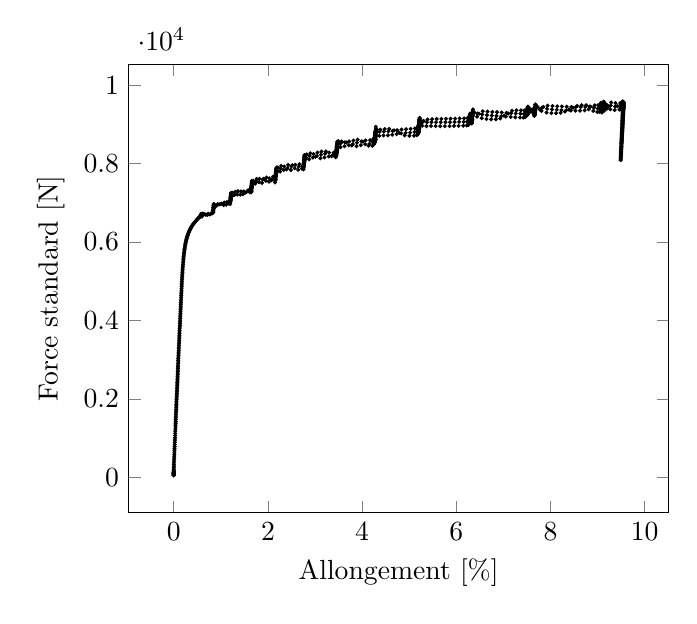
\begin{tikzpicture}
    \begin{axis}[
        xlabel={Allongement [\%]},
        ylabel={Force standard [N]}
    ]
        \addplot
[
    only marks,
    mark=*,
    mark size=0.5pt % Adjust the size here
]
 coordinates {
(5.50752496799946E-05,51.5997428894043)
(-0.000334300528164517,51.8629112243652)
(-0.000135359342302175,51.7863883972168)
(-0.000135356083962522,52.6386222839355)
(-0.000389994251439924,55.4920768737793)
(-0.00105007757153087,62.2801628112793)
(-0.00166187087243862,70.9940338134766)
(-0.00191651337467145,79.9237213134766)
(-0.00190060522953062,86.3036041259766)
(-0.00129692984913013,90.5912017822266)
(-0.000795257198863753,95.3709869384766)
(-0.000135760438095014,100.247940063477)
(0.000421024641834181,104.141426086426)
(0.000484905554426797,105.976875305176)
(0.000357749867694006,107.271987915039)
(0.000246184317970365,109.482009887695)
(-0.000110587109600431,113.485427856445)
(-0.000397616584304405,120.107498168945)
(-0.00062044000339301,128.586013793945)
(-0.000612516768680025,139.566482543945)
(-0.000755511331743703,156.343826293945)
(-0.000715662128708939,177.851638793945)
(-0.000350200702010128,202.761795043945)
(0.000405221607239479,235.449295043945)
(0.00099352501392599,274.918060302734)
(0.00259941353819903,318.644622802734)
(0.00399904264574878,365.777435302734)
(0.00553377834153903,414.441497802734)
(0.0069091570234817,465.246185302734)
(0.00892081356691713,517.191467285156)
(0.0105669193120518,569.847717285156)
(0.012514684004183,621.488342285156)
(0.0141927847828032,675.207092285156)
(0.0160927887322985,728.628967285156)
(0.0179296637474455,783.409851074219)
(0.0198458504735667,836.612976074219)
(0.0216427559016656,892.269226074219)
(0.0233763862356089,947.737976074219)
(0.0255309847431964,1003.14422607422)
(0.0277654535342702,1059.44116210937)
(0.0298168297035546,1115.89428710937)
(0.031836268558513,1172.81616210937)
(0.034174069540484,1227.51928710937)
(0.0355895369716106,1279.61303710937)
(0.0370844818235567,1328.21459960937)
(0.0385314676396252,1376.10522460937)
(0.0401775175275087,1422.73803710937)
(0.041624492172127,1469.26928710937)
(0.0433738593556408,1514.26147460937)
(0.0449155827935557,1558.26928710937)
(0.0463236323817234,1602.15209960937)
(0.0477155057099445,1645.05053710937)
(0.0495121132327037,1687.94116210937)
(0.0510229699536073,1730.87084960937)
(0.0523268271492093,1772.52941894531)
(0.053575348427959,1813.94348144531)
(0.0552927913305055,1855.26379394531)
(0.0565487267283974,1896.02160644531)
(0.0579803406289366,1936.34973144531)
(0.0594670670173232,1977.28723144531)
(0.0611211715208293,2018.08410644531)
(0.0622263481977412,2058.21704101562)
(0.0639040765946868,2099.25610351562)
(0.0650808920581669,2138.34204101562)
(0.0667033590145951,2177.74047851562)
(0.0685875432595973,2218.47485351562)
(0.0702647503221984,2258.44360351562)
(0.0716009004566256,2298.63110351562)
(0.0737715579239322,2337.92797851562)
(0.074884711016315,2376.50610351562)
(0.0765298709119961,2415.10766601562)
(0.0775723012767303,2453.46704101562)
(0.0792419415437026,2492.67016601562)
(0.0803468128676413,2531.93579101562)
(0.0814124053725384,2571.86767578125)
(0.0828118752869222,2611.73486328125)
(0.0843069057866535,2651.64892578125)
(0.0855634109285076,2691.89892578125)
(0.086787645474437,2731.83642578125)
(0.0879406657489072,2773.10205078125)
(0.0892523653025773,2814.41455078125)
(0.0908663494044571,2855.73486328125)
(0.0921787415880419,2897.72705078125)
(0.0933076836634297,2938.85986328125)
(0.0949059830491734,2980.57861328125)
(0.0964324276669777,3022.71923828125)
(0.0982372275865791,3064.03955078125)
(0.0997324144866137,3105.28173828125)
(0.101608778716448,3148.25830078125)
(0.102928424895055,3190.17236328125)
(0.104319903498701,3232.35986328125)
(0.105950205365564,3274.89111328125)
(0.107771233678547,3316.89892578125)
(0.109226315072222,3360.07861328125)
(0.110967735630799,3403.74169921875)
(0.112939005054233,3446.31982421875)
(0.114624955638555,3489.05419921875)
(0.116326561148479,3532.20263671875)
(0.117439900431699,3575.04638671875)
(0.119093617658263,3617.89794921875)
(0.120246585799299,3661.21044921875)
(0.12180509247929,3704.89013671875)
(0.123291878448745,3747.46044921875)
(0.125080561689468,3790.97607421875)
(0.128181160465232,3832.95263671875)
(0.130297003350031,3875.97607421875)
(0.131521349610463,3919.16357421875)
(0.132897076469271,3962.53857421875)
(0.135067793517646,4007.02294921875)
(0.136267696644954,4050.55419921875)
(0.137929770116297,4094.51513671875)
(0.139488485330026,4138.45263671875)
(0.14104712606742,4181.74951171875)
(0.143177983381341,4226.10107421875)
(0.144799690679153,4270.65869140625)
(0.145984251681466,4316.12744140625)
(0.147479423686233,4361.30712890625)
(0.149348213672806,4406.55712890625)
(0.151200767818363,4450.99462890625)
(0.152981750206055,4496.94775390625)
(0.155152258720691,4542.30712890625)
(0.156806258957328,4587.43994140625)
(0.158674721248027,4633.29150390625)
(0.1604003975094,4679.44775390625)
(0.162014359268379,4724.20556640625)
(0.163818891073175,4768.89306640625)
(0.165107540201185,4814.64306640625)
(0.166968108000381,4859.63525390625)
(0.168383322211969,4905.13525390625)
(0.170220266117725,4950.60400390625)
(0.17215230140792,4994.69775390625)
(0.174075935767534,5038.79931640625)
(0.176398167471688,5083.89306640625)
(0.178545156359754,5127.72119140625)
(0.180692115457286,5171.6669921875)
(0.183435138453789,5216.2998046875)
(0.185876293969558,5259.6435546875)
(0.188182155775295,5303.3857421875)
(0.190623072966792,5344.7451171875)
(0.193413909770319,5386.7451171875)
(0.196061394524375,5427.9482421875)
(0.198263659748226,5468.6826171875)
(0.200879506955204,5509.5029296875)
(0.203654912262134,5549.8076171875)
(0.206716425857327,5588.7529296875)
(0.209570597336078,5626.9326171875)
(0.212138958431906,5664.8388671875)
(0.215399353631893,5700.9560546875)
(0.218929651069664,5736.6748046875)
(0.223031807597553,5773.0732421875)
(0.226880804167752,5806.0966796875)
(0.23097545348108,5839.0263671875)
(0.235738364052459,5871.7529296875)
(0.240588739631579,5902.2763671875)
(0.244635172965675,5932.48291015625)
(0.248236491036434,5962.88916015625)
(0.252602815124316,5991.92822265625)
(0.258144807740121,6019.38916015625)
(0.263607200049153,6048.00244140625)
(0.270078180676328,6073.91650390625)
(0.275733138996953,6099.56494140625)
(0.281601159216543,6125.49853515625)
(0.287874569022418,6149.19775390625)
(0.293639156508058,6173.06884765625)
(0.300603468377803,6196.70166015625)
(0.307784655334861,6218.81494140625)
(0.316887689219495,6240.43994140625)
(0.324036464075591,6261.06884765625)
(0.330874464081297,6282.32666015625)
(0.33803896833933,6301.27978515625)
(0.346053813599049,6321.02978515625)
(0.353622992470553,6339.15869140625)
(0.361964341982601,6357.35400390625)
(0.36933523505999,6374.61181640625)
(0.37688802913781,6391.4365234375)
(0.385483908972111,6408.9208984375)
(0.394151286087944,6425.2958984375)
(0.403342976601678,6440.3623046875)
(0.412168601033968,6455.6767578125)
(0.421421302561275,6469.7177734375)
(0.431695938565944,6483.7412109375)
(0.441612134865866,6499.1396484375)
(0.450357682342841,6512.5302734375)
(0.459214765579005,6526.3193359375)
(0.468987967315864,6539.2822265625)
(0.478966127926447,6552.1318359375)
(0.488085367861561,6564.3935546875)
(0.49683282193271,6577.4853515625)
(0.506365792803622,6589.2451171875)
(0.516042711534684,6600.5517578125)
(0.524567094087454,6612.0087890625)
(0.532741616609261,6620.869140625)
(0.539579616614966,6630.748046875)
(0.547386166461156,6641.982421875)
(0.554082959335835,6649.97802734375)
(0.558949064316892,6642.28466796875)
(0.563115449236024,6655.82177734375)
(0.567599282085158,6678.35693359375)
(0.572799994343783,6689.87060546875)
(0.577952565099511,6706.34716796875)
(0.58594310128351,6715.64599609375)
(0.595882176713522,6648.40869140625)
(0.603458981961723,6684.01171875)
(0.612555342766747,6726.708984375)
(0.629594574901415,6696.9296875)
(0.647337340286356,6714.36376953125)
(0.678933418940906,6699.09423828125)
(0.708798310085299,6689.97998046875)
(0.729261785356798,6724.84521484375)
(0.764869338153828,6702.27783203125)
(0.790345249509253,6719.78173828125)
(0.815098561672663,6733.72607421875)
(0.826992372779756,6744.7607421875)
(0.830905776484401,6784.6357421875)
(0.832869806808081,6798.4931640625)
(0.833299922537563,6777.56640625)
(0.835087592900131,6798.3359375)
(0.837823198053675,6841.7626953125)
(0.834992382353557,6753.2392578125)
(0.838483177543281,6836.4423828125)
(0.839015832290694,6813.4833984375)
(0.841910340152442,6879.4365234375)
(0.842427146335782,6870.8984375)
(0.843571817813106,6889.46484375)
(0.84522549035387,6916.484375)
(0.846395066717595,6934.611328125)
(0.847134229446498,6939.97802734375)
(0.849320616315742,6968.75927734375)
(0.847778181628828,6884.9140625)
(0.849773968661722,6928.865234375)
(0.850601073046909,6910.6962890625)
(0.852914188847668,6962.9541015625)
(0.865938848624323,6879.5888671875)
(0.88098568984697,6931.8056640625)
(0.910059344409077,6930.2353515625)
(0.930119872918077,6965.1826171875)
(0.961788402151246,6959.8935546875)
(0.989386352822536,6965.34130859375)
(1.01726641985054,6980.39208984375)
(1.0564164246232,6943.19873046875)
(1.07200092540296,7009.96435546875)
(1.11601274531979,6952.2998046875)
(1.1312025811055,7021.3369140625)
(1.17161665781564,6975.8974609375)
(1.18277976670548,7022.4306640625)
(1.1957169614744,7017.3134765625)
(1.19988370387994,7065.6904296875)
(1.20105256527085,7056.9287109375)
(1.19900047412875,6970.6240234375)
(1.20116350521936,7027.5849609375)
(1.20247571865974,7049.3779296875)
(1.20412146691846,7076.7138671875)
(1.20669012591963,7128.5888671875)
(1.20407320625343,7051.58642578125)
(1.20638721577021,7111.13330078125)
(1.20855763491324,7089.619140625)
(1.21011699062345,7118.53173828125)
(1.20849519395404,7080.97509765625)
(1.21057814808933,7133.494140625)
(1.21087247856497,7136.90380859375)
(1.21188225850447,7169.55908203125)
(1.21132553300561,7145.1240234375)
(1.2137348722311,7202.5537109375)
(1.21231243381502,7157.4130859375)
(1.21317814673224,7178.16552734375)
(1.21620736738861,7241.02490234375)
(1.21692377014956,7254.0302734375)
(1.21314633044196,7153.4638671875)
(1.21749574840181,7228.5263671875)
(1.21642996225844,7190.03759765625)
(1.22041236083977,7246.77978515625)
(1.24304935346983,7178.17919921875)
(1.25298652230567,7255.82763671875)
(1.29398592342729,7203.84814453125)
(1.30485255692304,7282.64501953125)
(1.3502567863977,7211.66650390625)
(1.36056192790916,7295.68212890625)
(1.41106188780072,7207.4833984375)
(1.42299335414276,7291.0927734375)
(1.46782119636613,7220.1669921875)
(1.48365546098272,7291.5263671875)
(1.52004281079699,7261.1513671875)
(1.54781426153813,7279.2568359375)
(1.56913379759384,7314.2001953125)
(1.60645347195928,7279.0859375)
(1.61768712483356,7348.53515625)
(1.63949093580951,7274.865234375)
(1.64209272188446,7265.099609375)
(1.64386597362858,7292.3994140625)
(1.64466078507495,7292.17236328125)
(1.64679962625197,7336.03955078125)
(1.64598050572989,7294.4541015625)
(1.64856489413299,7356.3994140625)
(1.6473798266916,7313.3779296875)
(1.65009958328107,7369.2861328125)
(1.65146637297969,7393.10546875)
(1.65117347244968,7383.912109375)
(1.65289846352877,7423.876953125)
(1.65141310750495,7379.7705078125)
(1.65151403783404,7383.201171875)
(1.65126129494383,7374.47265625)
(1.65270744662495,7404.1171875)
(1.65375738420424,7432.1767578125)
(1.65303359339087,7417.1748046875)
(1.65393219505759,7434.9443359375)
(1.65355826427517,7416.3935546875)
(1.65809095360002,7459.68359375)
(1.65621331582486,7429.4765625)
(1.657654224372,7469.9951171875)
(1.65686572851884,7450.0849609375)
(1.65914839839388,7516.2626953125)
(1.65887754285901,7500.9521484375)
(1.66126293049518,7557.0146484375)
(1.65832951619607,7476.962890625)
(1.65910001856671,7502.375)
(1.66119977456316,7546.76416015625)
(1.65863898026296,7480.44970703125)
(1.66340117586153,7561.82470703125)
(1.68113297832997,7475.3466796875)
(1.68931417393138,7560.8154296875)
(1.73060337736748,7490.5517578125)
(1.7469219169043,7552.1884765625)
(1.76041679046917,7609.6904296875)
(1.80975182132031,7529.3984375)
(1.81997688587645,7615.9140625)
(1.87417754506011,7508.0478515625)
(1.88583827502941,7592.8212890625)
(1.9097431527853,7614.2822265625)
(1.95503811058135,7562.1962890625)
(1.9670496538787,7645.1337890625)
(2.02124649987401,7539.302734375)
(2.02960405543654,7625.787109375)
(2.07082271488819,7574.732421875)
(2.09324616897075,7606.08203125)
(2.10874868620102,7667.21630859375)
(2.14690178054486,7567.65380859375)
(2.15171283261914,7519.51416015625)
(2.1556239722432,7573.86083984375)
(2.15824959074532,7617.92529296875)
(2.15715091585245,7584.65966796875)
(2.16083231087852,7666.01904296875)
(2.158374710988,7588.53466796875)
(2.16178608461416,7672.58154296875)
(2.15944097377991,7593.31103515625)
(2.16305873622542,7676.10791015625)
(2.16072029847079,7604.18603515625)
(2.1640999749688,7682.34228515625)
(2.1643862024192,7673.91455078125)
(2.16727278599891,7737.80908203125)
(2.16549250368877,7678.599609375)
(2.16570628056055,7692.169921875)
(2.16772607876382,7728.3232421875)
(2.16782903484923,7672.74609375)
(2.17071585675321,7755.48046875)
(2.16705042945335,7663.58984375)
(2.17051709431055,7751.12890625)
(2.16713217467856,7671.7900390625)
(2.16870416157518,7714.2353515625)
(2.17153521559957,7774.408203125)
(2.16859262581599,7710)
(2.17248875101093,7797.421875)
(2.16860120548977,7700.4912109375)
(2.17135194423457,7774.36767578125)
(2.17255357521285,7798.42236328125)
(2.17336363941261,7757.93603515625)
(2.17566966506628,7818.18359375)
(2.17355429883003,7767.265625)
(2.17559792946048,7827.2734375)
(2.17656004454562,7850.91015625)
(2.17670327743296,7859.0966796875)
(2.17367369929018,7785.3681640625)
(2.17677477471449,7867.2587890625)
(2.17311697379132,7759.03369140625)
(2.17635270242918,7841.17822265625)
(2.18149717015967,7900.86962890625)
(2.20149495980413,7810.4912109375)
(2.20881723473007,7900.1318359375)
(2.25601116032361,7797.2021484375)
(2.26935922613706,7874.4814453125)
(2.2804479778541,7942.4931640625)
(2.33564769238503,7836.6416015625)
(2.34525311383456,7928.1259765625)
(2.39172634683026,7851.70068359375)
(2.41629662595295,7886.16259765625)
(2.42698117970506,7968.20947265625)
(2.48690543459962,7838.39501953125)
(2.49704184252666,7930.08251953125)
(2.51803535097858,7963.69189453125)
(2.57000338838427,7881.73486328125)
(2.58075276633831,7972.01611328125)
(2.6419735052713,7840.70751953125)
(2.65237016330312,7926.20751953125)
(2.66758859800144,7988.943359375)
(2.72170536704144,7870.71484375)
(2.73153957979187,7938.0419921875)
(2.74871513340999,7857.65185546875)
(2.75393967809579,7952.15185546875)
(2.75226235187106,7858.01513671875)
(2.75735915474719,7948.04638671875)
(2.75908557577191,7975.98779296875)
(2.75745424613163,7930.71044921875)
(2.76121571811302,8013.96044921875)
(2.75771640283058,7913.30615234375)
(2.76162039272649,8003.44677734375)
(2.75761392339372,7890.59716796875)
(2.76136657737705,7978.30029296875)
(2.76085132030148,7943.66748046875)
(2.76180247247012,7964.07470703125)
(2.76198836540211,7975.21728515625)
(2.7641177927704,8022.365234375)
(2.76728250077527,8080.05078125)
(2.76809327994784,8094.3076171875)
(2.76244785459808,7948.478515625)
(2.76597839036013,8042.087890625)
(2.76723650419081,8067.88818359375)
(2.76415687795097,7993.83447265625)
(2.76785471735179,8085.39697265625)
(2.76352150544242,7964.8505859375)
(2.76927012520185,8055.1630859375)
(2.77160093657979,8114.96044921875)
(2.7673682975131,8012.10400390625)
(2.7710275283819,8103.26025390625)
(2.76699651164914,7995.77978515625)
(2.76999391601523,8081.61962890625)
(2.77278469323768,8153.56103515625)
(2.76848317845646,8037.74072265625)
(2.77190980483601,8128.00634765625)
(2.76923938137079,8062.20361328125)
(2.77191004316028,8100.23876953125)
(2.77179946069818,8100.44384765625)
(2.7722036586631,8103.28564453125)
(2.77130755940124,8080.53173828125)
(2.77213978775827,8100.71142578125)
(2.77483595024483,8174.83447265625)
(2.7746057289983,8172.9208984375)
(2.7762673258211,8214.228515625)
(2.77051894438594,8065.865234375)
(2.77373894362186,8149.833984375)
(2.77656165629674,8221.716796875)
(2.77363455759083,8099.017578125)
(2.77902640591541,8193.705078125)
(2.79190163637367,8187.1689453125)
(2.81212678737339,8147.3720703125)
(2.82007061200013,8235.5908203125)
(2.87455916690408,8109.26953125)
(2.88491959964659,8198.29296875)
(2.89817996212803,8265.63671875)
(2.95597264473584,8154.23046875)
(2.96598417074448,8245.93359375)
(3.01081391956203,8178.0830078125)
(3.04039091498612,8192.1455078125)
(3.05073609497523,8282.2080078125)
(3.11373949946109,8136.25390625)
(3.12514283921687,8227.19140625)
(3.1364251102426,8307.52734375)
(3.20217401033928,8156.9580078125)
(3.21209783301589,8254.6298828125)
(3.22916757065735,8311.068359375)
(3.29174675793945,8184.412109375)
(3.30043796748246,8281.115234375)
(3.35071294926148,8190.1162109375)
(3.37743767980099,8213.7958984375)
(3.39085628959889,8278.1552734375)
(3.42773744730427,8179.9970703125)
(3.43437620821877,8275.7001953125)
(3.44091201304787,8163.8330078125)
(3.4462714492715,8248.6064453125)
(3.45120952818263,8330.1376953125)
(3.44705053131592,8208.1708984375)
(3.45124122531077,8302.9833984375)
(3.45142616494567,8288.3095703125)
(3.45055747297506,8255.232421875)
(3.45429392090791,8342.794921875)
(3.45011990961208,8215.587890625)
(3.45386446057018,8306.259765625)
(3.45428963107102,8310.5419921875)
(3.45325244384026,8264.9873046875)
(3.45673531474795,8354.4873046875)
(3.45315711413156,8236.708984375)
(3.45649722880045,8325.802734375)
(3.45579035901037,8297.46875)
(3.45912880540937,8366.2802734375)
(3.46208664794634,8407.189453125)
(3.46285000058883,8419.7666015625)
(3.463987522338,8449.1591796875)
(3.45679084430328,8270.693359375)
(3.46084593178749,8368.568359375)
(3.46520488271821,8409.2734375)
(3.46072700797587,8305.125)
(3.46442413240389,8399.6875)
(3.46030612731192,8299.8828125)
(3.46221415143174,8344.84375)
(3.46560884235887,8434.640625)
(3.46009115881878,8291.6640625)
(3.46366101808567,8385.0078125)
(3.46662672532361,8457.7919921875)
(3.46338289366051,8327.9287109375)
(3.46675399048474,8424.8974609375)
(3.46751853474858,8448.9287109375)
(3.4641698404059,8361.0888671875)
(3.46741438704182,8455.0419921875)
(3.46304137497906,8345.8251953125)
(3.46554497145403,8407.1572265625)
(3.46793917708826,8472.154296875)
(3.4659107992112,8382.66796875)
(3.46983909818284,8470.24609375)
(3.46606261177232,8376.5556640625)
(3.46931383148785,8464.2744140625)
(3.46941368935772,8465.0205078125)
(3.46788197926304,8427.2060546875)
(3.47128644148531,8516.5341796875)
(3.47057194531854,8494.982421875)
(3.47184269033563,8527.564453125)
(3.47345709895262,8562.369140625)
(3.46625327118974,8373.24609375)
(3.47069754220976,8470.1953125)
(3.47513466350163,8552.5859375)
(3.48070025022034,8397.47265625)
(3.48651297920888,8494.61328125)
(3.49557406802168,8570.7578125)
(3.53962735636179,8421.318359375)
(3.54692579886056,8521.333984375)
(3.56526628151911,8565.68359375)
(3.62619149835511,8443.642578125)
(3.63475591938553,8543.580078125)
(3.66704599831949,8536.486328125)
(3.71585099599021,8468.927734375)
(3.72543163171547,8566.380859375)
(3.77920521380411,8465.134765625)
(3.80413393263155,8498.3203125)
(3.81510447550979,8588.9765625)
(3.87931094091956,8444.2314453125)
(3.89115089074123,8534.3564453125)
(3.90442269278771,8612.7548828125)
(3.9717292803247,8471.1611328125)
(3.98418839660444,8568.3603515625)
(4.01632404141028,8560.8916015625)
(4.0637334121455,8496.1455078125)
(4.07318725935818,8593.3330078125)
(4.13518016893172,8458.9033203125)
(4.15673040288251,8505.966796875)
(4.16744736873559,8598.685546875)
(4.21838393869304,8453.66796875)
(4.227019857005,8550.41796875)
(4.23463765402795,8627.4609375)
(4.24794091487831,8492.8994140625)
(4.25381608482605,8590.8056640625)
(4.25703822898042,8619.5244140625)
(4.25426175121426,8532.7392578125)
(4.25866741370225,8627.3330078125)
(4.25572744548567,8526.97265625)
(4.25709304356292,8562.0859375)
(4.26127515788399,8649.5546875)
(4.25626605833987,8509.52734375)
(4.26029707507264,8600.74609375)
(4.26374848717645,8663.5712890625)
(4.25985998835821,8560.3251953125)
(4.26424896814717,8650.6064453125)
(4.26309786191451,8599.5986328125)
(4.26431998878016,8622.4619140625)
(4.26835195881001,8703.7431640625)
(4.26522705095853,8594.3681640625)
(4.26887579555937,8673.4931640625)
(4.27192205640117,8724.7841796875)
(4.27041918354337,8655.359375)
(4.27408461084324,8732)
(4.2759297173553,8744.7060546875)
(4.274689477845,8729.134765625)
(4.27709845958408,8782.595703125)
(4.27057838415692,8547.3310546875)
(4.27383008052098,8630.8466796875)
(4.27725718354908,8716.8154296875)
(4.27072948174522,8555.7685546875)
(4.27403694598888,8644.4091796875)
(4.2772814926248,8732.0341796875)
(4.27086437328304,8570.978515625)
(4.27650026566193,8668.009765625)
(4.27976197164541,8750.955078125)
(4.27315419288624,8588.8359375)
(4.27705079472972,8686.1640625)
(4.27989733983178,8762.796875)
(4.27401263691316,8612.6943359375)
(4.27778149694698,8712.2724609375)
(4.28033490319475,8777.5673828125)
(4.27704269170448,8638.3203125)
(4.28042165322968,8735.0234375)
(4.28004414758319,8728.0810546875)
(4.27778912332367,8666.5966796875)
(4.2809702757033,8760.3623046875)
(4.27648644285416,8636.4150390625)
(4.27912516919123,8711.8095703125)
(4.28199650001755,8792.7470703125)
(4.27812420724979,8680.15625)
(4.28130440633232,8765.671875)
(4.28357849653358,8819.6025390625)
(4.28092261084894,8739.34765625)
(4.28488213030018,8821.06640625)
(4.28431062869646,8804.998046875)
(4.28377725897624,8800.7509765625)
(4.28432588144986,8801.8037109375)
(4.28543122942234,8834.6435546875)
(4.28370528504616,8795.82421875)
(4.28718863260239,8877.82421875)
(4.2900828425588,8939.94921875)
(4.29301613769578,8613.1806640625)
(4.30084842656332,8709.7900390625)
(4.30679461714405,8807.2275390625)
(4.31658402493139,8869.33984375)
(4.3637503049094,8709.6328125)
(4.37133568983139,8808.8984375)
(4.38731676219938,8866.673828125)
(4.45406853083168,8718.095703125)
(4.46263104526794,8816.501953125)
(4.4778980981177,8882.80078125)
(4.54871281893518,8722.236328125)
(4.55764187610142,8822.0517578125)
(4.57396804201495,8884.6708984375)
(4.6403098928998,8737.0771484375)
(4.64985239674158,8835.2490234375)
(4.67822823783594,8847.9189453125)
(4.73314196324074,8753.4189453125)
(4.74273975831357,8851.6064453125)
(4.78972586514212,8787.6259765625)
(4.82694258342216,8772.8525390625)
(4.83736593377242,8870.3994140625)
(4.90331883944573,8722.2255859375)
(4.92259641314089,8782.7919921875)
(4.93217704886616,8878.9169921875)
(5.00376584691836,8710.373046875)
(5.01777359431607,8792.2607421875)
(5.02889475813408,8886.4951171875)
(5.10125382023265,8712.9677734375)
(5.11143884631113,8806.3115234375)
(5.12040841860357,8898.2177734375)
(5.16063374249047,8727.7216796875)
(5.1682896713969,8820.12890625)
(5.17477876466873,8913.53515625)
(5.18030455123405,8743.130859375)
(5.18593329388478,8835.904296875)
(5.19132514220937,8925.607421875)
(5.18560821957809,8760.0751953125)
(5.18987756058262,8852.8408203125)
(5.19391715698917,8936.5908203125)
(5.18793807765894,8776.7587890625)
(5.19209683620137,8873.5712890625)
(5.19612022655744,8950.0283203125)
(5.1907288548814,8799.2109375)
(5.1949672137306,8894.9609375)
(5.19859307920136,8967.568359375)
(5.19436282337739,8835.9453125)
(5.19863121108484,8928.2421875)
(5.20176565190719,8982.703125)
(5.19906925109636,8917.181640625)
(5.20383287664055,8979.275390625)
(5.20347539023289,8961.583984375)
(5.20417463364627,8963.6171875)
(5.20602736653504,9010.6484375)
(5.20573422768076,8984.849609375)
(5.20644872384753,8998.673828125)
(5.20856361343524,9046.283203125)
(5.20737103877929,9000.42578125)
(5.20838868341976,9023.560546875)
(5.21086153606368,9077.037109375)
(5.21298452867663,9115.294921875)
(5.20007974600867,8793.3583984375)
(5.20393583272596,8883.8740234375)
(5.20756980122195,8974.7333984375)
(5.20182189643533,8824.0322265625)
(5.20550209984005,8890.26171875)
(5.20909602985838,8981.90234375)
(5.2020678470838,8807.125)
(5.20535100225174,8897.796875)
(5.20917515351661,8991.65625)
(5.2029577499146,8816.9619140625)
(5.20791155822767,8904.3115234375)
(5.21147402944213,8999.458984375)
(5.20458073820538,8832.572265625)
(5.2072518766434,8909.705078125)
(5.21105219548109,9007.486328125)
(5.2051403235955,8854.7265625)
(5.20755407182001,8922.0068359375)
(5.2115612561256,9018.0224609375)
(5.206672748663,8883.9287109375)
(5.20953311657281,8929.65625)
(5.21399407029186,9027.890625)
(5.20691822266292,8871.1328125)
(5.20999498901151,8940.90625)
(5.21342113874252,9035.296875)
(5.20710935872888,8881.896484375)
(5.21053550845989,8963.607421875)
(5.2141051294025,9053.638671875)
(5.20975666473974,8929.044921875)
(5.2137876814725,9006.048828125)
(5.21688065387157,9087.376953125)
(5.21426528331313,9016.994140625)
(5.21610943652811,9064.0498046875)
(5.2175651211801,9108.98828125)
(5.21579151194957,9058.0205078125)
(5.21796169276833,9114.7783203125)
(5.21864663672541,9128.6416015625)
(5.21813709943236,9113.2490234375)
(5.22044312508603,9163.7412109375)
(5.22121481907803,9163.1220703125)
(5.21976819074837,9128.5576171875)
(5.22410855238589,8981.4248046875)
(5.23054902750628,9055.2060546875)
(5.24944718896078,9037.66796875)
(5.27477390932207,8967.265625)
(5.28363003926115,9062.390625)
(5.30465977300238,9093.48828125)
(5.36642675116628,8957.72265625)
(5.37509412828211,9057.80078125)
(5.3895251395865,9126.982421875)
(5.46204054240735,8959.1767578125)
(5.47153538139478,9057.8486328125)
(5.48523426053628,9134.2744140625)
(5.55981831803612,8956.291015625)
(5.56986797592824,9056.150390625)
(5.58238286008757,9139.501953125)
(5.65821383017733,8956.171875)
(5.66894032900128,9056.421875)
(5.68194139467502,9141.984375)
(5.75758742512988,8957.330078125)
(5.7677038138181,9056.892578125)
(5.77953995045142,9144.705078125)
(5.85639857480106,8957.0361328125)
(5.86613173806026,9057.4267578125)
(5.87815472092266,9145.8173828125)
(5.95218014632946,8962.6435546875)
(5.96232513393028,9060.7373046875)
(5.97466651801977,9148.0185546875)
(6.04884447096051,8965.19921875)
(6.05946610710488,9065.13671875)
(6.07130415033237,9152.94921875)
(6.14779670860057,8968.35546875)
(6.1565822945552,9065.63671875)
(6.1669031654686,9155.2314453125)
(6.21981878017885,8973.3759765625)
(6.22802571480162,9067.5166015625)
(6.23573788823619,9160.0478515625)
(6.25146538357902,8986.8525390625)
(6.25823188630319,9075.0791015625)
(6.264545572911,9164.9384765625)
(6.26086441620919,8998.2216796875)
(6.26508656900792,9084.0029296875)
(6.27027107521607,9171.3935546875)
(6.26439447532269,9008.6630859375)
(6.2684817365836,9098.3037109375)
(6.27290217517644,9180.7802734375)
(6.26763902195861,9024.8994140625)
(6.27175774202339,9114.4306640625)
(6.27619438666671,9198.7119140625)
(6.27133638471089,9036.7041015625)
(6.2752715950864,9121.7900390625)
(6.27989174941899,9208.6337890625)
(6.27976496090641,9141.482421875)
(6.28172017323203,9166.9765625)
(6.28568016933181,9227.875)
(6.28585557599583,9190.67578125)
(6.2859985705589,9176.529296875)
(6.28861441776588,9227.662109375)
(6.29129365922915,9272.380859375)
(6.29235181899582,9259.927734375)
(6.29712164097108,9228.546875)
(6.30380854338848,9241.9853515625)
(6.3107189939728,9264.3251953125)
(6.32099934975999,9255.529296875)
(6.32880017982366,9214.810546875)
(6.32486353950252,9087.5341796875)
(6.32923583659246,9179.3779296875)
(6.33300612657191,9254.6591796875)
(6.32600892595266,9047.9013671875)
(6.33030209938437,9142.8857421875)
(6.33406333304149,9232.5419921875)
(6.32569100137411,9030.4697265625)
(6.32947559080987,9124.3447265625)
(6.33351518721641,9216.6982421875)
(6.32661331630587,9031.4501953125)
(6.33118532913556,9121.9033203125)
(6.33494560949559,9217.4345703125)
(6.32732971906682,9035.5615234375)
(6.33111335520549,9119.2177734375)
(6.33487458886261,9217.1865234375)
(6.32930924046817,9077.3505859375)
(6.33251136538371,9116.5576171875)
(6.33649614720775,9215.7294921875)
(6.33391271210173,9158.755859375)
(6.3320833349916,9113.158203125)
(6.33674257450476,9212.939453125)
(6.33871017969252,9238.9150390625)
(6.33474780035002,9112.1689453125)
(6.33829358886546,9209.5283203125)
(6.3411892287675,9268.865234375)
(6.33465199399277,9121.78515625)
(6.33862771949448,9219.31640625)
(6.34160248305475,9277.771484375)
(6.335502811643,9137.3466796875)
(6.33986795900479,9230.7998046875)
(6.34237322374967,9283.28125)
(6.33837223587514,9158.181640625)
(6.34253147106612,9245.212890625)
(6.3433675126115,9261.361328125)
(6.3406386996997,9198.630859375)
(6.34394664059191,9274.693359375)
(6.34465494032762,9275.1044921875)
(6.3425958186195,9218.271484375)
(6.34486943217221,9271.298828125)
(6.34771597727427,9329.869140625)
(6.34710491384144,9308.873046875)
(6.34665829415614,9262.5439453125)
(6.34978320200763,9324.4892578125)
(6.35249437892331,9379.8330078125)
(6.34688136567452,9247.5810546875)
(6.34885278405062,9300.2216796875)
(6.35266120591355,9380.5810546875)
(6.38514623410182,9305.24609375)
(6.43839693273819,9195.107421875)
(6.4495543218455,9276.138671875)
(6.4798615428383,9274.47265625)
(6.53773430240144,9158.87890625)
(6.54817481209926,9255.25390625)
(6.56091848755949,9335.94921875)
(6.64098209671593,9139.83203125)
(6.65081630946637,9238.39453125)
(6.66215482502023,9327.81640625)
(6.74075226325672,9131.423828125)
(6.75252166909395,9225.798828125)
(6.76399364624001,9318.923828125)
(6.84016589668694,9132.580078125)
(6.85344532511012,9219.021484375)
(6.86375237321575,9314.021484375)
(6.9331295220259,9151.859375)
(6.95343284338677,9209.76953125)
(6.96320604512363,9305.97265625)
(7.01397102160541,9222.544921875)
(7.05361674086335,9199.5703125)
(7.06405153077865,9297.716796875)
(7.09985546277562,9280.052734375)
(7.15405230877093,9190.802734375)
(7.16394371934659,9287.599609375)
(7.18184091885964,9349.509765625)
(7.25232961207334,9181.529296875)
(7.26216573141794,9281.060546875)
(7.27696471539795,9359.435546875)
(7.35199872912289,9178.982421875)
(7.36193017817621,9274.826171875)
(7.37203417400229,9359.638671875)
(7.42480870074366,9176.337890625)
(7.43397560553313,9268.275390625)
(7.44315204329347,9357.072265625)
(7.46190911677907,9188.0439453125)
(7.46942300441953,9270.2939453125)
(7.47676053209887,9356.5283203125)
(7.47655557322514,9207.7587890625)
(7.48194551495556,9279.8779296875)
(7.48779685247612,9363.0029296875)
(7.48676586167643,9252.79296875)
(7.49033357602487,9303.3798828125)
(7.49522494337874,9366.7822265625)
(7.49739607749459,9284.56640625)
(7.49965396164536,9292.427734375)
(7.50316018833168,9350.927734375)
(7.50607060433857,9364.4384765625)
(7.50249192707363,9254.5888671875)
(7.50668929414809,9340.3388671875)
(7.51116693056616,9418.1669921875)
(7.51146960239131,9383.65625)
(7.51323415529952,9403.2890625)
(7.51001439438787,9298.869140625)
(7.51258210009195,9360.1767578125)
(7.51666936135285,9435.0048828125)
(7.5126002127366,9310.4453125)
(7.51275703010743,9305.439453125)
(7.51696393015276,9391.955078125)
(7.52053355109538,9453.62109375)
(7.5151669651436,9314.6875)
(7.51765554718945,9370.7841796875)
(7.52100304991077,9433.4208984375)
(7.51422844416135,9263.4970703125)
(7.5185931148746,9359.5595703125)
(7.52315750132759,9447.9189453125)
(7.51510404753585,9246.8408203125)
(7.51885527157355,9329.6806640625)
(7.523101733448,9416.0166015625)
(7.51942010009765,9313.4765625)
(7.52376999470605,9408.7734375)
(7.53193212436572,9427.3095703125)
(7.5575300577483,9319.9033203125)
(7.57158737659454,9336.6962890625)
(7.58320997468036,9385.6884765625)
(7.61231604134343,9318.6552734375)
(7.63498353948028,9304.2109375)
(7.64386540844071,9386.6953125)
(7.65099845389487,9394.90234375)
(7.65400372296193,9263.9990234375)
(7.65900376618372,9360.5302734375)
(7.66378359777839,9438.9951171875)
(7.65565769340803,9244.1982421875)
(7.65971254256797,9342.5576171875)
(7.66366443564251,9426.5732421875)
(7.65531593640231,9234.1806640625)
(7.65957765103015,9329.9775390625)
(7.66356052626001,9416.3369140625)
(7.65619678291078,9227.1201171875)
(7.66104858843553,9323.9169921875)
(7.66497617243434,9411.6044921875)
(7.65704045083285,9223.095703125)
(7.66102427935981,9318.126953125)
(7.6650314636654,9407.908203125)
(7.65769298268897,9225.33203125)
(7.66182790880423,9315.76953125)
(7.66605006160295,9406.48828125)
(7.65887840761677,9232.5048828125)
(7.66246375796132,9314.2392578125)
(7.66636750953295,9404.3642578125)
(7.66069110202787,9251.8720703125)
(7.66359913479204,9312.12109375)
(7.66782986726455,9404.08984375)
(7.66291705072623,9286.662109375)
(7.66463393878008,9320.416015625)
(7.66852196094978,9408.291015625)
(7.66566874276812,9331.146484375)
(7.66603337890393,9335.296875)
(7.66973932133,9414.5625)
(7.66721880383173,9347.1611328125)
(7.66655054257368,9325.001953125)
(7.66894427155936,9381.744140625)
(7.66839660238283,9366.0615234375)
(7.66564395704385,9294.7314453125)
(7.66958774709315,9381.9658203125)
(7.67266451344173,9451.3251953125)
(7.66529362036435,9268.7705078125)
(7.66961920589702,9363.1923828125)
(7.67377033806276,9454.1142578125)
(7.67124410078197,9387.7705078125)
(7.66987421286782,9350.8212890625)
(7.67400103595784,9443.615234375)
(7.67729277079956,9510.775390625)
(7.66922215766025,9266.267578125)
(7.67280798465334,9361.720703125)
(7.67679133653175,9454.876953125)
(7.67862119029042,9498.64453125)
(7.67164734544981,9338.525390625)
(7.67527988400017,9426.150390625)
(7.67914455039124,9505.634765625)
(7.67135420659553,9324.41796875)
(7.67507349518081,9407.83984375)
(7.67896104070197,9497.33984375)
(7.69647024830058,9465.5458984375)
(7.72472978715031,9448.521484375)
(7.76903903575831,9384.080078125)
(7.80982871152076,9343.93359375)
(7.82179068336958,9428.41796875)
(7.84813028188591,9446.603515625)
(7.9160126608635,9303.3203125)
(7.92646842331472,9398.0234375)
(7.9388798747401,9480.845703125)
(8.01760314819209,9288.2177734375)
(8.03038876872416,9382.3740234375)
(8.04204759209928,9470.5771484375)
(8.11805206225889,9287.8349609375)
(8.13105503452681,9374.8193359375)
(8.14217619834482,9465.3505859375)
(8.21453716703756,9293.4208984375)
(8.23089097856661,9366.0380859375)
(8.24226667270687,9459.2099609375)
(8.30481630777927,9329.2236328125)
(8.33144952179843,9361.0166015625)
(8.34297679017553,9453.7666015625)
(8.39256158486349,9377.5322265625)
(8.43175544130216,9354.2001953125)
(8.44265353360179,9446.2314453125)
(8.47869007008801,9427.94140625)
(8.52962664004546,9352.34765625)
(8.53966867156088,9444.03515625)
(8.56460311017084,9473.5556640625)
(8.62753787726643,9350.0986328125)
(8.63967144259092,9440.6298828125)
(8.66038277510506,9490.603515625)
(8.72409161943537,9357.8125)
(8.73750450945074,9444.34375)
(8.75780211102909,9491.599609375)
(8.81015337386379,9386.029296875)
(8.82577981971539,9455.498046875)
(8.85225287982391,9453.83984375)
(8.90847834202055,9344.9404296875)
(8.92201325406307,9425.3935546875)
(8.93735943057106,9488.8447265625)
(8.99347812349394,9317.4931640625)
(9.00371272102096,9405.9462890625)
(9.01274425762406,9491.4150390625)
(9.03729165761665,9322.2294921875)
(9.04639564479838,9394.216796875)
(9.05343097730111,9487.951171875)
(9.0592289301848,9518.94921875)
(9.059745617206,9384.072265625)
(9.06682098818639,9476.697265625)
(9.07276860871275,9552.564453125)
(9.08961050835039,9303.951171875)
(9.09641704955222,9396.654296875)
(9.1034933738297,9492.248046875)
(9.11288335013755,9535.7607421875)
(9.11100630817307,9379.4443359375)
(9.11530091155041,9468.2568359375)
(9.12017416625962,9547.4755859375)
(9.11336762505779,9349.4658203125)
(9.11775660484676,9438.8564453125)
(9.12233719735023,9530.8095703125)
(9.11782238234577,9399.212890625)
(9.11985671832962,9433.275390625)
(9.12428478329916,9525.431640625)
(9.12702265253329,9563.267578125)
(9.12077093023614,9406.703125)
(9.12492921213003,9501.03125)
(9.12900932366279,9582.046875)
(9.12127999088065,9375.880859375)
(9.1256851767201,9473.6806640625)
(9.12958892829174,9551.2119140625)
(9.12416657446036,9411.1162109375)
(9.12812657056014,9503.6630859375)
(9.12847071080858,9450.0654296875)
(9.1286022658066,9458.0927734375)
(9.13238780853944,9554.5771484375)
(9.13047549458273,9507.5830078125)
(9.1291999830802,9475.47265625)
(9.13214185789097,9542.177734375)
(9.12885774942594,9461.044921875)
(9.13239638821322,9536.185546875)
(9.13297789943635,9543.109375)
(9.1306699671885,9470.5869140625)
(9.13371575138175,9542.0869140625)
(9.12994164821396,9462.9306640625)
(9.13032868683132,9460.1259765625)
(9.13412852902047,9545.7666015625)
(9.13000361252462,9446.3544921875)
(9.13296074008878,9466.3544921875)
(9.13676058227792,9553.6748046875)
(9.1327891466131,9468.0986328125)
(9.13287303675676,9469.1416015625)
(9.13648984590519,9556.8759765625)
(9.1333430122207,9483.78125)
(9.1328558774092,9471.888671875)
(9.1364745931518,9549.669921875)
(9.12869854881239,9370.68359375)
(9.13342976225563,9435.388671875)
(9.13703894502735,9522.654296875)
(9.13040113740994,9376.33203125)
(9.13268905041896,9426.50390625)
(9.1364669667751,9517.50390625)
(9.12962420028396,9364.119140625)
(9.13190258032211,9413.7197265625)
(9.13586257642188,9506.9384765625)
(9.1345765786514,9472.328125)
(9.13223718759968,9405.89453125)
(9.13618860402567,9500.70703125)
(9.13765191505435,9529.3828125)
(9.13136968725042,9387.57421875)
(9.13590166160246,9482.27734375)
(9.13934592397811,9553.384765625)
(9.13129056359219,9370.869140625)
(9.13553464222392,9465.666015625)
(9.13902752275103,9545.986328125)
(9.13250697067532,9359.9462890625)
(9.13624484855381,9453.7431640625)
(9.13966337190812,9535.2119140625)
(9.13234014368508,9361.2109375)
(9.13633922496543,9449.4921875)
(9.13956804219941,9528.40625)
(9.13187970119202,9371.8759765625)
(9.13559946642585,9451.0400390625)
(9.13858995938805,9522.8916015625)
(9.13331822649644,9390.779296875)
(9.13730968140009,9431.9072265625)
(9.13994936103424,9501.2041015625)
(9.13357371011578,9353.4501953125)
(9.13518668878714,9399.6376953125)
(9.13862904456862,9490.533203125)
(9.13655657670129,9446.9462890625)
(9.13370812500506,9388.1455078125)
(9.13758709085243,9480.5517578125)
(9.13847937692595,9506.7509765625)
(9.13382728714094,9399.1376953125)
(9.13757183809904,9489.2783203125)
(9.13882923695691,9511.2666015625)
(9.13518668878714,9380.689453125)
(9.13862999786571,9462.220703125)
(9.14156424629978,9528.267578125)
(9.13338209740127,9349.9638671875)
(9.13684923890702,9433.6044921875)
(9.14085594656407,9522.1201171875)
(9.14307522218282,9377.3837890625)
(9.14790748511728,9408.2578125)
(9.15359390224178,9498.3984375)
(9.17572088093025,9426.248046875)
(9.19303942911144,9400.904296875)
(9.20041890186261,9493.232421875)
(9.23116940600091,9456.3798828125)
(9.27059491363174,9386.1787109375)
(9.27828420793622,9481.7099609375)
(9.28829382735068,9562.6318359375)
(9.36233450551087,9368.2431640625)
(9.37209245449434,9457.3056640625)
(9.38194382659234,9547.0087890625)
(9.42234265054909,9467.75)
(9.46152125423436,9377.2294921875)
(9.47008376867062,9470.7451171875)
(9.48004667652781,9548.2998046875)
(9.49776084300014,9379.845703125)
(9.5056503296929,9445.04296875)
(9.51569903428793,9533.69921875)
(9.51779628787953,9466.7294921875)
(9.51888971963843,9427.111328125)
(9.52409853492229,9517.923828125)
(9.52932260295955,9584.099609375)
(9.52269909479844,9414.4130859375)
(9.52673058817975,9498.2255859375)
(9.53095274097848,9578.26953125)
(9.52347889181568,9389.54296875)
(9.52612619782653,9440.5908203125)
(9.53018057033793,9527.3720703125)
(9.53400424495426,9547.76171875)
(9.53558767141591,9473.7861328125)
(9.53723401548532,9511.7802734375)
(9.53873736499166,9537.23828125)
(9.53432359947843,9425.591796875)
(9.53760008156676,9503.529296875)
(9.54100335216768,9575.013671875)
(9.53345705242626,9405.521484375)
(9.53710722697274,9489.177734375)
(9.54158391009372,9573.037109375)
(9.53609005898081,9438.84765625)
(9.53872878531788,9435.0478515625)
(9.54250574837693,9522.2666015625)
(9.54448574642682,9565.5185546875)
(9.54105864339873,9505.0029296875)
(9.54121784401227,9510.2978515625)
(9.54088419003179,9512.869140625)
(9.53929409049053,9482.8056640625)
(9.5419175640742,9531.3994140625)
(9.53859532372569,9462.5888671875)
(9.53907769205176,9473.1044921875)
(9.54224359167798,9549.5888671875)
(9.53595469079444,9399.2958984375)
(9.53932459599731,9471.7080078125)
(9.54539233195665,9554.7705078125)
(9.53771161732595,9396.2900390625)
(9.54140755013261,9475.7353515625)
(9.54551912046923,9561.1572265625)
(9.53853907919755,9400.9404296875)
(9.54170211893252,9466.4697265625)
(9.54535229347899,9554.5322265625)
(9.54187180581402,9485.5263671875)
(9.53975453298359,9449.609375)
(9.54364207850475,9536.03125)
(9.5456544886556,9576.2578125)
(9.54261728413612,9449.36328125)
(9.54543237043431,9520.33203125)
(9.54707871450371,9563.984375)
(9.53887177988094,9389.3759765625)
(9.54260107808564,9476.1728515625)
(9.54641712632527,9555.5791015625)
(9.53802048558217,9382.0986328125)
(9.54156770404324,9462.8408203125)
(9.54587660687689,9548.9501953125)
(9.53974690660689,9405.7548828125)
(9.54267257536718,9466.9970703125)
(9.54648957690389,9551.5283203125)
(9.5423160422566,9468.1943359375)
(9.54144854190735,9455.3642578125)
(9.54580510959536,9538.7392578125)
(9.54570310680704,9516.1201171875)
(9.54369069665619,9450.5771484375)
(9.54640187357188,9517.2646484375)
(9.54318163601168,9454.2900390625)
(9.54266399569339,9445.048828125)
(9.54551816717214,9521.845703125)
(9.54268306163513,9454.9033203125)
(9.541718324983,9435.92578125)
(9.54553532651971,9522.42578125)
(9.54532369456638,9521.4453125)
(9.54043042061834,9412.283203125)
(9.54668023632131,9495.251953125)
(9.54780131369573,9534.283203125)
(9.54175836346066,9410.5078125)
(9.54516068076448,9490.4765625)
(9.5470939672571,9540.3388671875)
(9.54174215741017,9417.3779296875)
(9.54423884248127,9478.5654296875)
(9.54481177403061,9500.48828125)
(9.54105864339873,9418.166015625)
(9.54394522697844,9481.283203125)
(9.54346953173198,9474.859375)
(9.54216351472267,9439.0205078125)
(9.54707776120662,9492.1455078125)
(9.54462969428697,9449.3525390625)
(9.54394522697844,9434.859375)
(9.546370414768,9490.23828125)
(9.54285751500207,9421.009765625)
(9.54299860297096,9430.703125)
(9.54593285140503,9498.0078125)
(9.54093185488615,9388.2236328125)
(9.5421320559188,9417.61328125)
(9.54527316982076,9486.80078125)
(9.54047141239308,9379.9638671875)
(9.54312443818646,9415.3642578125)
(9.54784135217338,9486.9736328125)
(9.54156770404324,9366.5556640625)
(9.54376124064063,9419.208984375)
(9.54545620286148,9462.06640625)
(9.54063728608624,9361.150390625)
(9.54330079814757,9420.423828125)
(9.54360489991835,9430.96484375)
(9.54082031912696,9376.423828125)
(9.54355532846982,9433.564453125)
(9.54105101702203,9382.609375)
(9.54071640974446,9374.107421875)
(9.54594905745551,9432.763671875)
(9.54145616828405,9342.296875)
(9.54302243539814,9389.95703125)
(9.54257057257886,9397.48046875)
(9.53962774447101,9339.4609375)
(9.54263253688952,9402.8046875)
(9.53873736499166,9318.5185546875)
(9.54003289573302,9351.2119140625)
(9.54226742410516,9397.072265625)
(9.53875261774506,9301.845703125)
(9.54230650928573,9362.947265625)
(9.53983460993891,9318.376953125)
(9.53988132149617,9323.466796875)
(9.54206151193435,9369.25)
(9.53783077946184,9278.068359375)
(9.54008056058738,9338.189453125)
(9.53782410638223,9294.21484375)
(9.53795661467734,9295.0712890625)
(9.54072498941825,9345.6845703125)
(9.53719397700766,9252.34765625)
(9.540470459096,9309.1328125)
(9.53800713942295,9263.453125)
(9.53834651318596,9268.8671875)
(9.54044662666882,9315.890625)
(9.53609673206042,9222.7734375)
(9.53842659014127,9285.5546875)
(9.53531788834027,9219.404296875)
(9.53645517176517,9248.0341796875)
(9.54022450844753,9278.3623046875)
(9.53650283661952,9199.185546875)
(9.5393179229177,9262.544921875)
(9.53515106135003,9179.2626953125)
(9.5369403999825,9227.6083984375)
(9.53628929807201,9222.2626953125)
(9.53428356100077,9176.82421875)
(9.53649521024282,9237.73046875)
(9.53248659599161,9145.7099609375)
(9.53463342103174,9203.4287109375)
(9.53257525262071,9156.330078125)
(9.53547708895381,9160.9228515625)
(9.53562866319066,9172.876953125)
(9.53360862666311,9132.876953125)
(9.53496040193261,9172.6259765625)
(9.53174016437241,9102.625)
(9.53366391789416,9150.85546875)
(9.53067533152613,9088.869140625)
(9.531866952885,9122.060546875)
(9.53084215851637,9100.0205078125)
(9.53009382030301,9084.9140625)
(9.53094511460178,9104.82421875)
(9.53174016437241,9060.3857421875)
(9.53256762624401,9094.4423828125)
(9.52963337780994,9036.708984375)
(9.53085741126977,9070.275390625)
(9.52879066318495,9025.1962890625)
(9.52916340234601,9038.8330078125)
(9.5285361328627,9026.240234375)
(9.52745414066885,9009.9248046875)
(9.5277086709911,9018.05859375)
(9.52612619782653,8985.1572265625)
(9.52727110762813,9004.9482421875)
(9.52765337976005,8959.3759765625)
(9.52830543496762,8986.26171875)
(9.52596795051008,8940.0400390625)
(9.52682591788846,8960.9599609375)
(9.52478300223082,8927.1298828125)
(9.52462380161728,8930.0341796875)
(9.52394028760583,8916.2158203125)
(9.52333589725262,8905.0498046875)
(9.52287450146247,8905.8916015625)
(9.52163426195216,8874.2392578125)
(9.52238164686844,8895.2724609375)
(9.52135494590564,8842.5498046875)
(9.52353418304673,8872.7314453125)
(9.52130823434837,8826.970703125)
(9.52164188832886,8841.9755859375)
(9.52037781639137,8814.7392578125)
(9.51958276662074,8810.3447265625)
(9.51887542018212,8795.68359375)
(9.51830248863278,8785.294921875)
(9.51768284552617,8773.4326171875)
(9.51679913912643,8760.515625)
(9.51570284747628,8741.6376953125)
(9.51596500417523,8742.623046875)
(9.51616424326643,8707.6787109375)
(9.51639398786442,8721.7041015625)
(9.51419187159324,8681.8310546875)
(9.51461322890573,8697.3671875)
(9.5123634477802,8655.173828125)
(9.51293542603245,8669.3251953125)
(9.51052644429337,8622.697265625)
(9.511551238662,8642.7373046875)
(9.50944445209953,8599.8720703125)
(9.51307842059552,8610.9892578125)
(9.51085247189716,8577.2333984375)
(9.51088297740395,8583.8818359375)
(9.50876189138517,8543.3544921875)
(9.50939678724517,8561.1357421875)
(9.50690010217408,8511.615234375)
(9.50774281679907,8533.888671875)
(9.50495251622515,8474.458984375)
(9.50651878333924,8509.85546875)
(9.50352066400034,8445.98828125)
(9.50453115891266,8477.513671875)
(9.50226421843955,8419.49609375)
(9.50575519237248,8439.2734375)
(9.5030363890801,8393.0634765625)
(9.50294868574809,8398.87890625)
(9.50104781135643,8355.783203125)
(9.50132617410586,8371.966796875)
(9.49923559359387,8325.5400390625)
(9.49905256055314,8318.5908203125)
(9.49840908501936,8307.9716796875)
(9.4958799878473,8266.8115234375)
(9.4968256585577,8280.41015625)
(9.49498770177379,8232.0947265625)
(9.4971211806547,8239.6396484375)
(9.49545005086103,8204.8134765625)
(9.49440047076814,8192.0439453125)
(9.49321647578597,8168.7109375)
(9.49219072812026,8150.115234375)
(9.4913165546914,8132.21875)
(9.48982083156175,8093.2109375)
(9.48950338363175,8092.09716796875)
};
    \end{axis}
\end{tikzpicture}

\end{figure}

\subsection{Résistance à la traction (force maximale avant rupture)}

\textbf{Fibre de carbone} : Avec une résistance maximale de \textbf{21 149 N $\pm$ 106}, la fibre de carbone se distingue par une capacité à supporter des charges élevées, soit environ \textbf{2 fois plus} que la fibre de verre et \textbf{2,2 fois plus} que l’aluminium.

\textbf{Fibre de verre} : La fibre de verre supporte une force maximale de \textbf{10 286 N $\pm$ 52}, ce qui la place au second rang, mais elle reste bien en deçà de la fibre de carbone en termes de performance.

\textbf{Aluminium} : L’aluminium, avec une force maximale de \textbf{9 584 N $\pm$ 48}, affiche une résistance légèrement inférieure à celle de la fibre de verre.

\subsection{Allongement maximal avant rupture}

\textbf{Fibre de verre} : L’allongement maximal de \textbf{1,84 \% $\pm$ 0,01} montre que ce matériau est plus ductile que la fibre de carbone, mais reste bien moins élastique que l’aluminium.

\textbf{Fibre de carbone} : Avec un allongement de seulement \textbf{0,673 \% $\pm$ 0,003}, la fibre de carbone est très rigide et casse après une faible déformation, ce qui peut limiter son usage dans des applications nécessitant flexibilité ou absorption d’énergie.

\textbf{Aluminium} : L’aluminium affiche une capacité d’allongement bien supérieure, à \textbf{9,54 \% $\pm$ 0,05}, témoignant d’une grande ductilité. Cela le rend idéal pour des applications où une déformation importante est nécessaire avant rupture.


\section{Perspectives avec la masse des matériaux}
La masse étant un paramètre primordial et une contrainte importante dans l'aéronautique, il est important de la prendre en compte.
Ainsi, afin d'obtenir une donnée plus pertinente dans ce cadre particulier, nous avons voulu comparer le rapport entre les performances mécaniques des matériaux et leur masse volumique.
Nous avons donc coupé des échantillons de composite à renfort en de fibre de verre et en fibre de carbone et mesurer leurs dimensions ainsi que leur masse :
\begin{table}[h!]
    \centering
    \begin{tabular}{|c|c|c|c|c|}
        \hline
        \textbf{Matériau} & \textbf{Longueur (mm)} & \textbf{Largeur (mm)} & \textbf{Épaisseur (mm)} & \textbf{Masse (g)} \\ \hline
        Fibre de carbone  & 21,9                   & 29                    & 4,51                    & 4,076              \\ \hline
        Fibre de verre    & 22,46                  & 30,29                 & 2,86                    & 2,67               \\ \hline
    \end{tabular}
    \caption{Dimensions et masse des matériaux analysés}
    \label{tab:dimensions_masse}
\end{table}

\noindent
A l'aide de la formule du volume : \[ V=L\cdot l\cdot h \] \\
Et de la masse volumique : \[\rho = \frac{M}{V}\]
On obtient:
\[
    V_{carbone} = 22.46\cdot 30.29 \cdot 2.86 = 1938.27 \unit{10} \\
    V_{verre} = 22.46\cdot 30.29 \cdot 2.86 = 1938.27 mm^3
\]
